\documentclass{WileyMSP-template}

\usepackage{chemformula} % Formula subscripts using \ch{}
\usepackage[T1]{fontenc} % Use modern font encodings
\usepackage{hyperref}
\usepackage{subfig}
\usepackage{caption}
\usepackage{enumitem}
\usepackage{graphicx}
\usepackage{amssymb}
\usepackage[style=numeric,backend=biber,sorting=none]{biblatex}
\usepackage{xr}
\externaldocument{Supplementary}
\usepackage{booktabs}
\usepackage[style=numeric,backend=biber]{biblatex}
\addbibresource{template.bib}
\begin{document} 
   
  
\pagestyle{fancy}
\rhead{\includegraphics[width=2.5cm]{vch-logo.png}}


\title{Attention-based pattern discovery of mass spectrometry imaging data }
\maketitle

 

% Author: Please give full first and last names for authors and include * after the name of all corresponding authors

\author{Guoqing Jiang}
\author{Xuemeng Fan}
\author{Ran Huang}
\author{Cong Wu*}   
\author{Bairong Shen*}



% Dedication

%\dedication{Optional dedication here. If no dedication is required, please leave blank}






% Affiliations: Please provide adacemic titles (Prof. or Dr.) for all authors where applicable, and include an institutional email address for all corresponding authors
\begin{affiliations}
Prof. C. Wu, Prof. B. Shen\\
Department of Urology and Institutes
for Systems Genetics, West China Hospital, Sichuan
University, Chengdu 610041, China\\
Email Address: congwu@wchscu.cn, bairong.shen@scu.edu.cn
\end{affiliations}


% Keywords: Please provide a minimum of three and a maximum of seven keywords, separated by commas

\keywords{mass spectrometry imaging, attention mechanism, neural network}



% Abstract should be written in the present tense and impersonal style (i.e., avoid we), and be at most 200 words long
\begin{abstract}
Mass spectrometry imaging (MSI) enables the direct 
visualization of molecular distributions in tissue sections, 
making it a crucial method in metabolomics research. 
However, the vast size and high dimensionality of MSI data  pose challenges 
for analysis even though there are already many 
conventional machine learning methods used in this area, such as the 
"Curse of dimensionality" problem. 
Therefore, compressing sparse distributions of raw data 
while ensuring minimal information loss 
is important.   
In response to these challenges, 
we propose Atnal, an attention-based generative model. 
Atnal effectively maps MSI data to a low-dimensional 
space with an extremely low loss ($2 \times 10^{-7} \sim 7 \times 10^{-9}$), 
which can contribute to the pattern discovery of MSI data. 
Then Atnal is applied in the domain of cancer region recognition 
and correlation analysis, based on the metabolomics 
data collected from patients with prostate cancer and colorectal adenocarcinoma. 
As it is presented, 
Atnal can distinguish 
the regions primarily containing cancer 
cells from those with normal cells and 
identify highly correlated metabolites with cancer 
(correlation coefficient up to 0.79). 
Atnal can provide quantitative guidance for the clinical removal of cancerous tissue, 
helping to avoid subjective bias 
and further aid in clinical cancer diagnosis. 
\end{abstract} 
\begin{figure}[ht!]
  \centering
  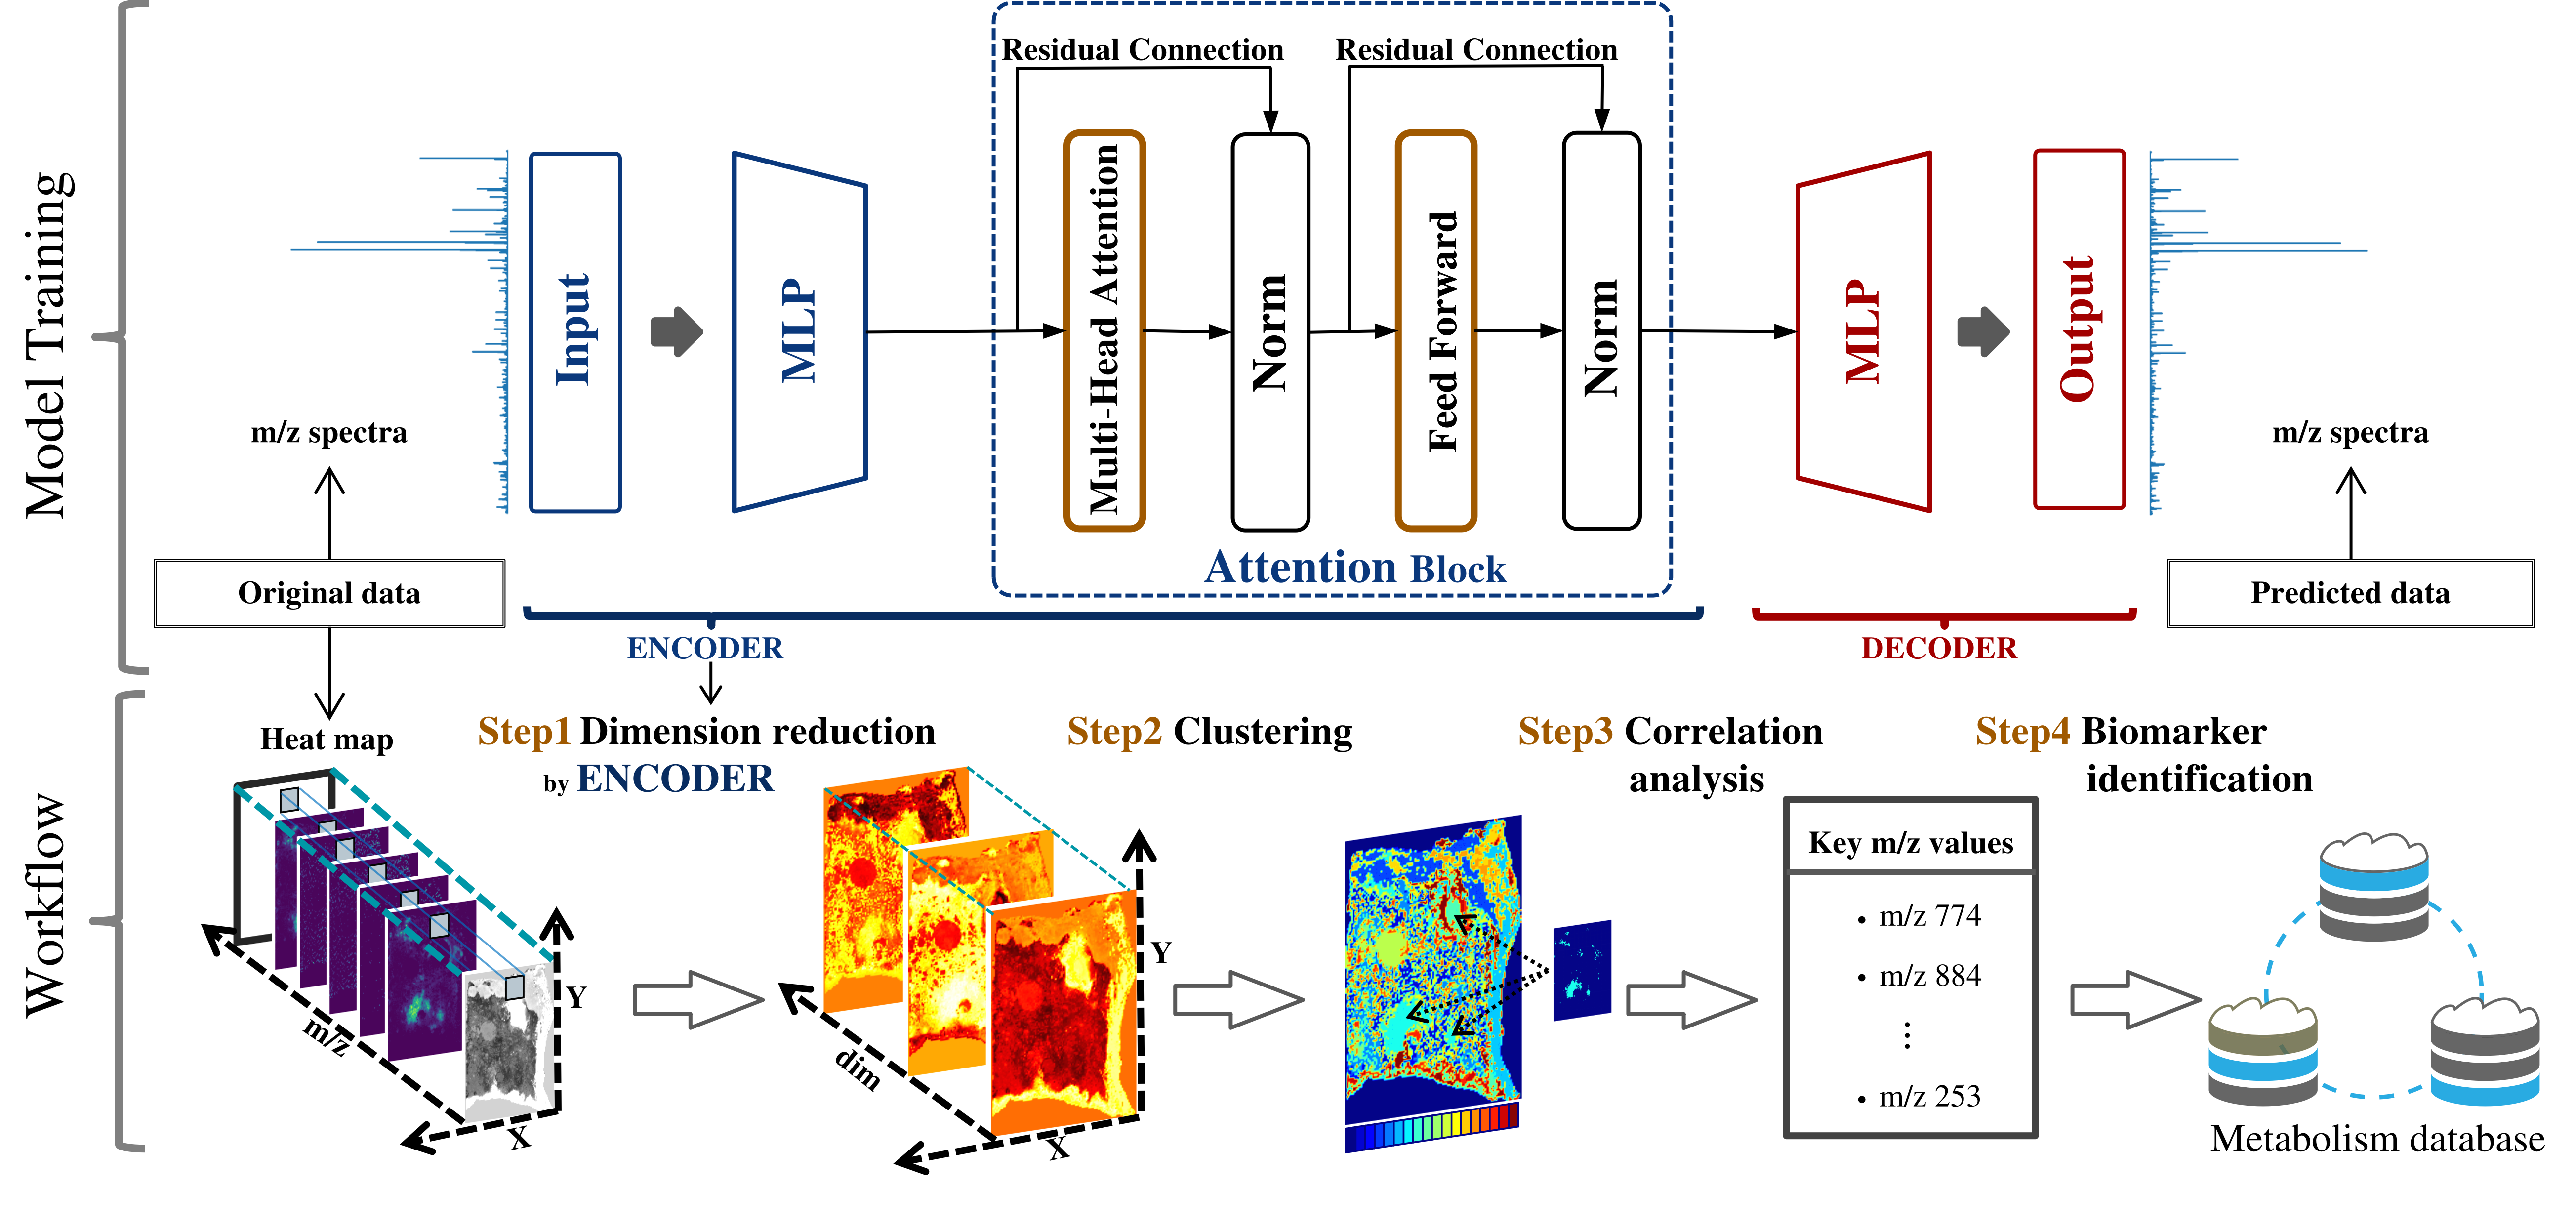
\includegraphics[width=\textwidth]{./pic/workflow.png}
  \captionsetup{justification=raggedright,singlelinecheck=false}
  \caption
    {
      \textbf{Training process and workflow of Atnal}. 
      During the training, 
      Atnal undergoes iterative unsupervised training,  
      which means the model's loss is 
      determined by the original and predicted data. 
      As for the workflow, 
      a 3D 'Heat map' is created 
      for clearly visualizing what each step does, despite 
      the data in the 'Heat map' actually remaining 
      in a 2D format, essentially the same as 'm/z spectra'.  
    }
  \label{fig:Atnal woskflow}
\end{figure} 

\section{Introduction}
Mass spectrometry imaging (MSI) is an analytical technique that effectively 
portrays the spatial distribution of molecules by combining mass spectrometry 
analysis with spatial imaging. This approach allows for the direct 
visualization of molecular distributions in solid samples or tissue sections. 
  

% MSI experiments are conducted by acquiring mass spectrometry on a virtual pixel 
% grid on the sample surface. In these experiments, complex molecular mixtures are 
% desorbed from the sample and ionized for MS analysis [1-3, 7, 8]. Various 
% desorption/ionization techniques, such as laser ablation, cluster beam, charged 
% droplets, or small liquid volume desorption, have been integrated with MSI. 
% A typical MSI experiment generates hundreds of thousands of mass spectra, 
% each containing thousands of different m/z features. Subsequently, 
% these features are extracted and visualized as a two-dimensional heat map, 
% illustrating the spatial distribution of molecules in the sample.

% However, the highly complexity  of MSI data hinders effective data 
% clustering and visualization, and classification using conventional machine learning 
% techniques [10, 11]. This data complexity poses challenges in terms of memory and 
% computation, primarily due to the "curse of dimensionality",  where the original 
% MSI data contains tens of thousands of spectra, with each spectrum 
% having $10^4$ to $10^6$ m/z spectral bins, and the nonlinear separability of the 
% underlying spectral manifold in high-dimensional space.


Mass spectrometry imaging data analysis poses various challenges. 
For example, the obtained data is usually vast, 
particularly when employing high-resolution and high-sensitivity instruments, 
thus making manual data preprocessing a bottleneck 
in the overall analysis process. 
Moreover, mass spectrometry imaging data, 
characterized by its high dimensionality, 
usually encompasses thousands of mass-to-charge ratio (m/z) channels, 
which leads to sparse data distribution in high-dimensional space and data complexity. 
This phenomenon is known as the "Curse of dimensionality" problem.  
As a consequence, 
the utilization of conventional machine learning methods for 
tasks like visualization and clustering 
is impeded in dealing with MSI data. 

As the common dimensionality reduction methods, 
principal component analysis (PCA) and non-negative matrix factorization (NNMF) 
are usually used for MSI data 
analysis \cite{race2013memory} \cite{jones2011multiple}. 
However, they can only present the 
linear mapping relations, which, 
in turn, hinders the capturing of complex 
nonlinear manifolds within the spectra. 

In contrast, t-distributed stochastic neighbor embedding (t-SNE) and 
uniform manifold approximation and projection (UMAP), 
as nonlinear dimensionality reduction methods, 
become increasingly favored in omics data analysis over the past years 
\cite{van2008visualizing} \cite{shekhar2014automatic} \cite{inglese2017deep}. 
Nevertheless, t-SNE can not project 
unseen data into the computed embedding. 
Additionally, the embedding results in t-SNE 
may undergo significant changes 
due to minor variations in the original data distribution. 
When it comes to UMAP, there are certain parameters that need to be 
adjusted, such as the number of neighbors and the minimum distance of points. 
In practical application, it is necessary to 
experiment with various combinations of these parameters to obtain 
the best result, which may introduce subjectivity. 
All of these problems may adversely affect the versatility 
and stability of the analysis. 

As for another unsupervised method, self-organizing 
maps (SOMs) \cite{nobile2023unsupervised}  can 
cluster sample regions containing benign cells and those containing malignant 
cells into distinct classes. However, due to the multiple iterations 
on the entire dataset, it can be time-consuming to train SOMs. 
Furthermore, the boundaries of true 
clusters in high-dimensional space may not be clear or may overlap, 
which makes the clusters derived from  
SOMs do not fully correspond to the true clusters of the original data.
 
% Furthermore, another approach \cite{janssen2022multimodal} 
% involves multimodal learning, where mass 
% spectrometry data and stained images are jointly input into a neural network 
% to directly identify cancerous regions. This method bypasses the process of 
% dimensionality reduction and clustering. 
% However, this method relies on a supervised learning mode that necessitates strict 
% data annotation, which potentially increases the 
% burden on annotators and introduces subjective bias. 
% Moreover, it is not tested on datasets of which 
% optical images fail to maintain consistent shape with the MSI data 
% due to distortions. 
  
With the development of deep learning, the encoder-decoder architecture 
emerges as a promising tool in the field of bioinformatics.  
By designing appropriate encoder layers, it is possible to achieve efficient 
data compression while minimizing the loss of essential information. 
Based on this architecture, msiPL \cite{abdelmoula2021peak}
is constructed by using
variational autoencoders (VAEs). 
However, the backpropagation-based threshold analysis of msiPL
may mistakenly exclude some crucial biomarkers. 

In this context, we propose a novel neural network architecture 
called Atnal, to extend the unsupervised encoder-decoder framework. 
As the kernel of Atnal, the attention mechanism is widely applied 
in other fields, such as medical image 
processing \cite{sinha2020multi}, natural language processing \cite{devlin2018bert}, 
computer vision \cite{liu2021swin}, and shows  
impressive capabilities. 
As an unsupervised generative model, Atnal allows for nonlinear mapping 
from high-dimensional to low-dimensional spaces without any labels.
Atnal eliminates the manual  peak picking process \cite{abdelmoula2021peak}
and remains independent of the properties of samples and mass spectrometers 
(ion sources and analyzers). 
Moreover, through reducing information loss caused by dimensionality reduction (two 
to three orders of magnitude, see Figure \ref{fig:model performance}b), 
Atnal achieves significant improvements without 
substantial increasing the number of parameters. 

In summary, our key contributions are as follows:
\begin{enumerate}[label=\roman*.]
  \item We propose an attention-based autoencoder model (Atnal) that greatly 
  enhances the feature extraction capability for metabolomic MSI data by using 
  unsupervised learning. To the best of our knowledge, this is the first 
  unsupervised learning approach to 
  employ the attention mechanism for encoding raw MSI metabolomic data. 
  \item Atnal eliminates the need for manual peak picking, thus reducing subjectivity 
  in the encoded features and clustering results, 
  while also minimizing the possibility of missing crucial biomarkers.
  \item Experimental results demonstrate that Atnal significantly outperforms 
  existing MSI dimensionality reduction methods, achieving state-of-the-art 
  results and validating the effectiveness 
  of our approach in metabolomic data analysis.
\end{enumerate}
% Text: Please use section headings and subheadings as specified below. For communications, all section headings apart from Experimental Section should be removed
% Please make the first reference to a display item bold: \textbf{Figure 1}
% Do not abbreviate Figure, Equation, etc.; display items are always singular, i.e., Figure 1 and 2.
% Equations are always singular, i.e., Equation 1 and 2, and should be inserted using the {equation} environment, not as graphics
% Please do not use footnotes in the text, additional information can be added to the Reference list.

\section{Results and discussion}

\subsection{Hyperparameters and implementation details}
The original MSI data is analyzed via Atnal, an encoder-decoder model 
based on attention mechanism and multi-layer perceptron 
(MLP), as depicted in Figure \ref{fig:Atnal woskflow}. 




The proposed 
neural network architecture is comprised of five layers: an $Input$ 
layer ($L_1$), three hidden layers: $MLP_e (h_2)$, $Attention \, BLock (h_3)$ and 
$MLP_d (h_4)$,  
and an $Output$ layer ($L_5$). 
As shown in Table \ref{tbl:Dimensions of Each Layer}, 
the number of artificial neurons of $L_1$ or $L_5$ 
is the same as that of m/z  bins, and  the dimension of the output from 
hidden layers $h_2$, $h_3$, and $h_4$ 
is 256, 256 and m/z dimensions, respectively. 
The $Attention \, Block$ ($h_3$) contributes to capturing the encoded features that represent 
the non-linear dimensionality reduction 
of original MSI data. Layers $h_2$, $h_3$, and $h_4$ 
are performed by batch normalization on their output. Further, 
the rectified linear unit \cite{nair2010rectified} (ReLU) function is used for neuron activation 
in the output of hidden layers $h_2$ and $h_4$. As for the $Output$ layer $L_5$, its neurons
are activated by the softmax function. 

From a macro view in Atnal, the unsupervised learning process involves minimizing 
the reconstruction error between the original and predicted data. 
The minimization is realized through  
optimizing the cost function which is modeled as the marginal likelihood and  
calculated via categorical cross-entropy; The Adam stochastic gradient optimizer 
is employed with a learning rate of 0.0002, in which the training is performed 
on mini batches consisting of 512 spectra for a total of 20 epochs. 
\begin{table}[htbp]
  \centering
  \caption{ \textbf{Dimensions of the output of each layer}}
  \begin{tabular}{ccccccc}
    \toprule
    \textbf{Input} & \multicolumn{2}{c}{\textbf{MLP$_e$}} & \textbf{Attention Block} & \multicolumn{2}{c}{\textbf{MLP$_d$}} & \textbf{Output}\\
    \cmidrule(r){1-1} \cmidrule(lr){2-3} \cmidrule(lr){4-4} \cmidrule(l){5-6}\cmidrule(l){7-7}
     & \textbf{Linear$_{e1}$} & \textbf{Linear$_{e2}$} &  & \textbf{Linear$_{d1}$} & \textbf{Linear$_{d2}$}& \\
    \midrule
    m/z dim & 512 & 256 & 256 &  512 & m/z dim &m/z dim\\
    \bottomrule
  \end{tabular}
  \label{tbl:Dimensions of Each Layer}
\end{table}
\begin{figure}[ht!]
  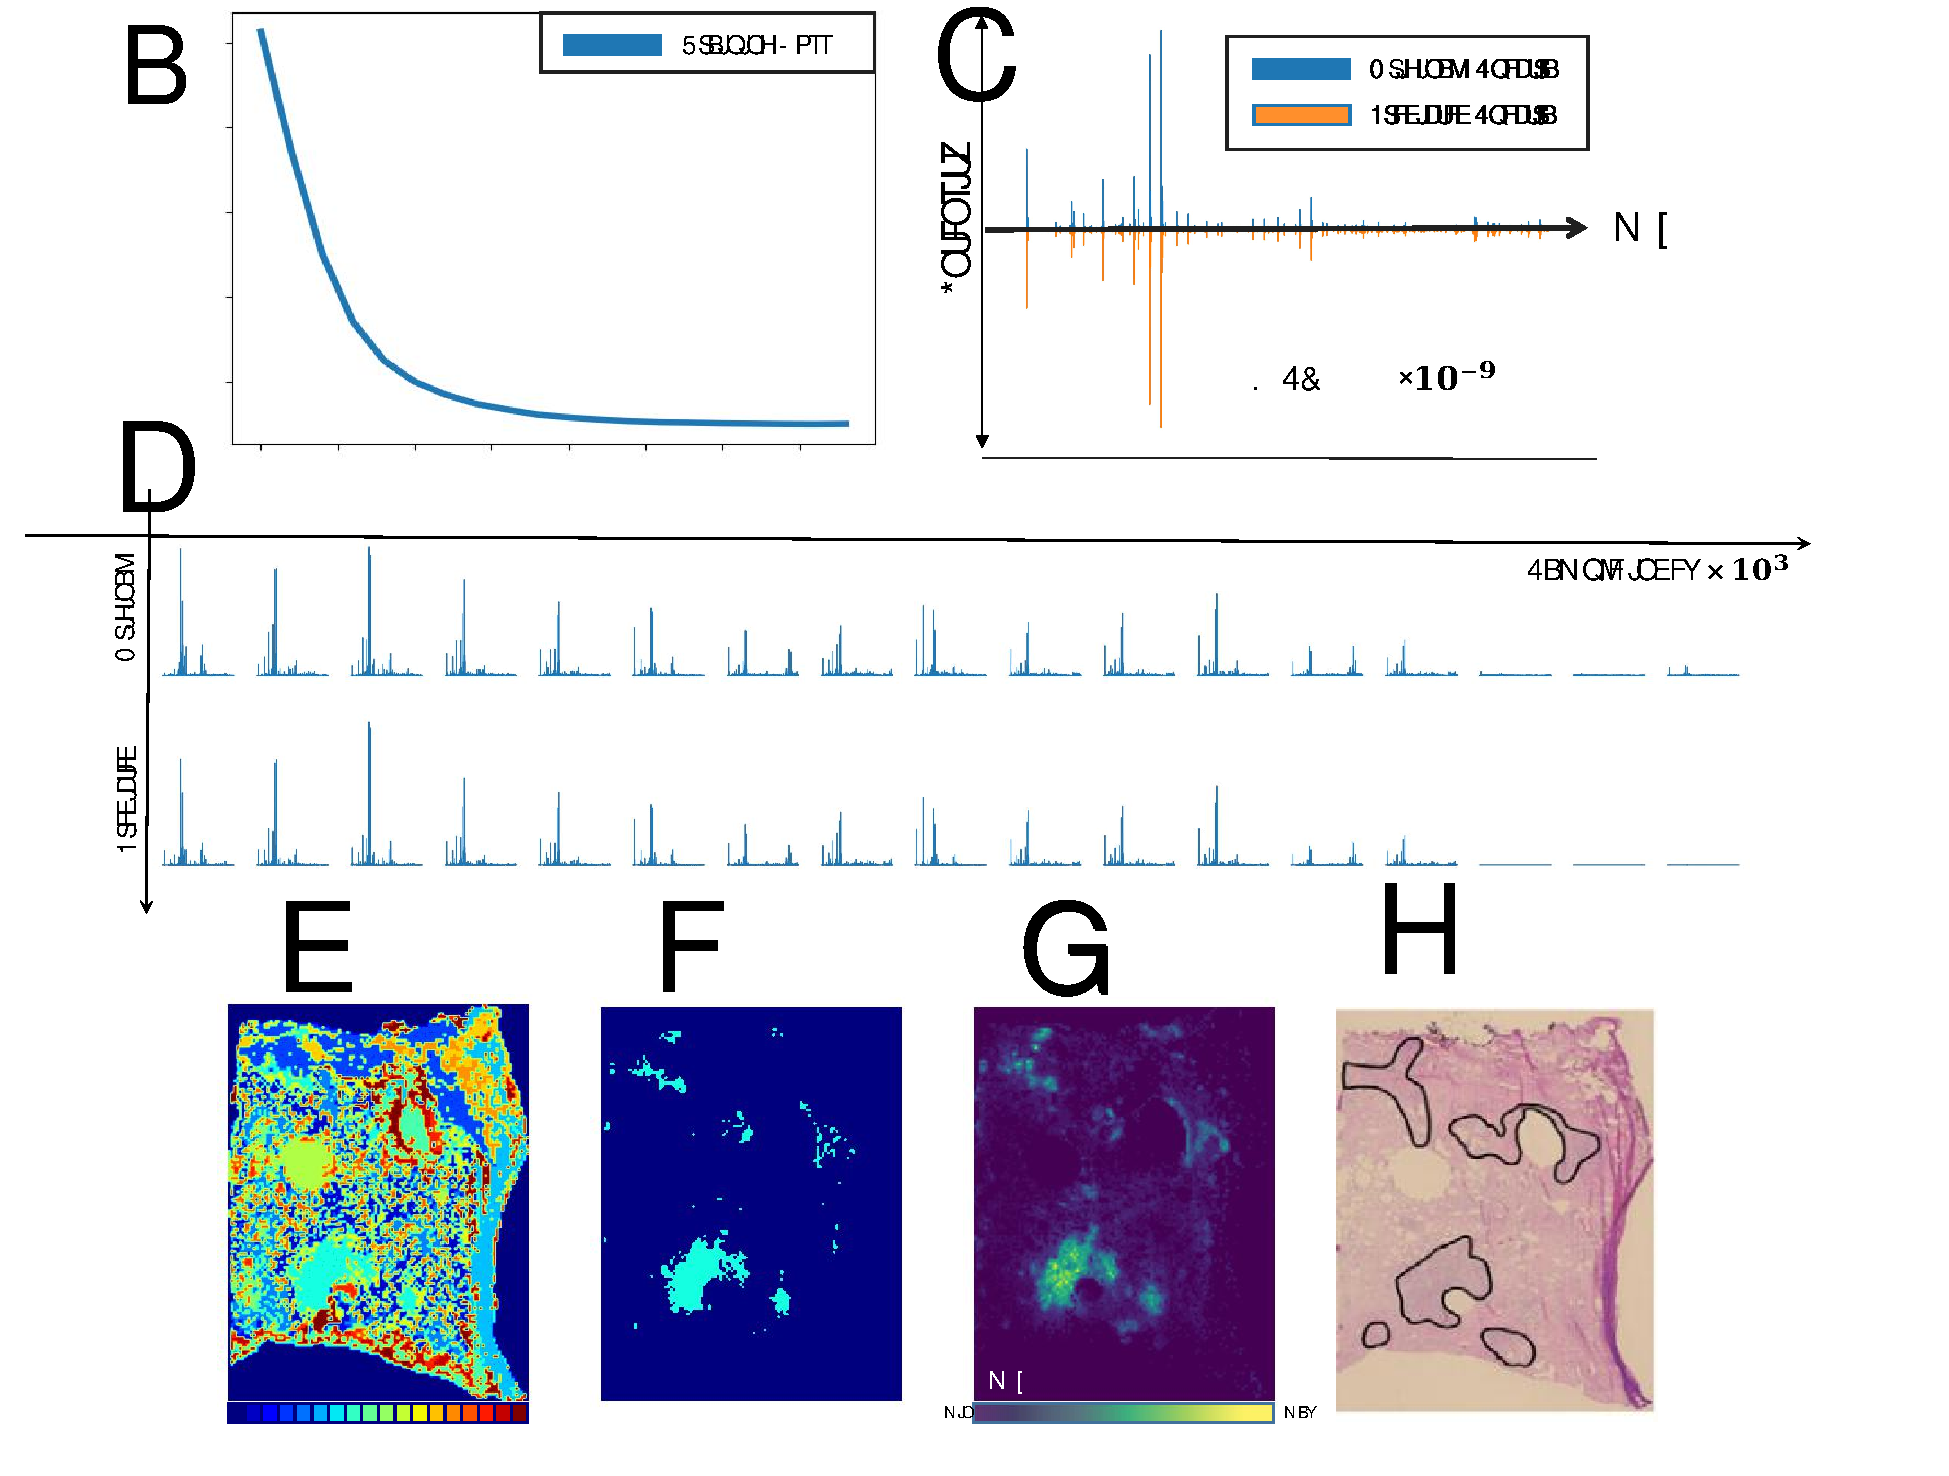
\includegraphics[width=\textwidth]{./pic/prostate.pdf}
  \captionsetup{justification=raggedright,singlelinecheck=false}
  \caption
    {
      \textbf{Analysis on prostate cancer dataset}. 
      (a): Training loss curve spanning 20 epochs. 
      (b): Mean Squared Error (MSE) averaged across all spectra. 
      (c): Reconstruction results of some spectra. 
      (d): Clustering outcomes of encoded features compressed by Atnal's encoder. 
      (e): Chosen cluster associated with cancer. 
      (f): Molecular pattern of m/z value that exhibits the highest correlation with (e). 
      (g): Histopathological annotation of tumor regions. 
      H\&E images of tissue post-MALDI MS imaging, Gleason score (GS) is indicated inset and tumor regions as determined by histopathologic evaluation are marked in black \cite{randall2019molecular}. 
    } 
  \label{fig:Prostate}
\end{figure}

\begin{figure}[]
  \centering
  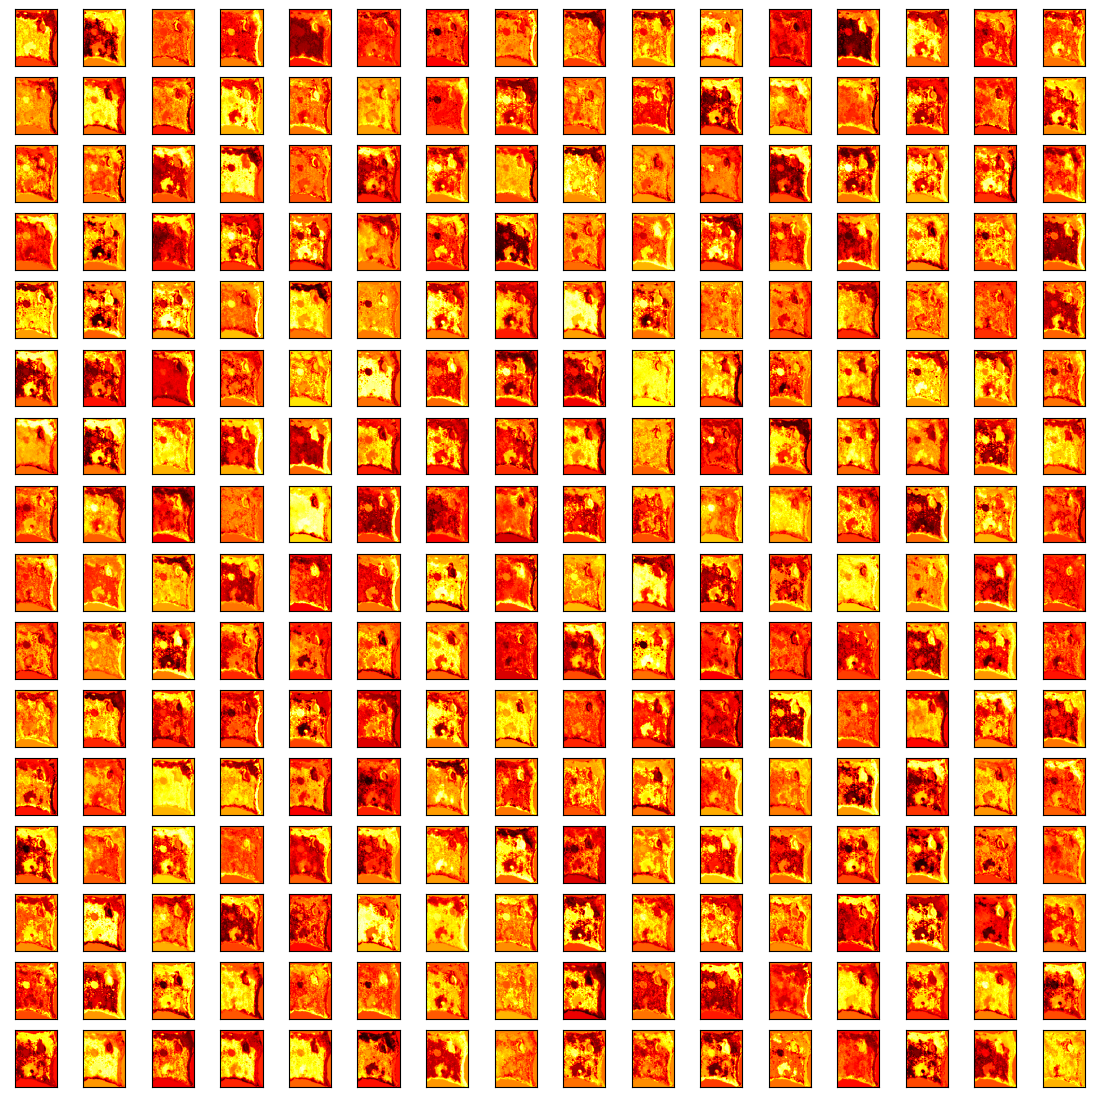
\includegraphics[width=\textwidth]{pic/encoder_feature_2D_train_pro.png}
  \captionsetup{justification=raggedright,singlelinecheck=false}
  \caption
  {
    \textbf{256-dimentional encoded features of MSI data from the prostate cancer dataset.}
    The original high-dimensional data is compressed 
    into 256 dimensions with minimal error, significantly 
    enhancing the information on each dimension 
    (see Supplementary Figure \ref{fig:Several   patterns of prostate tissue} 
    for comparison). Furthermore, 
    the distinctions between various zones within the prostate 
    cancer tissue become discernible, 
    thereby establishing a foundational basis for subsequent analyses. 
  }
  \label{fig:encoder_feature_2D_train_pro}
\end{figure}
 

\begin{table}[ht]
  \centering
  \caption{ \textbf{Identified compounds in the prostate cancer dataset}}
  \label{tbl:Compounds_pro}
  \begin{tabular}{|p{4cm}|p{12cm}|c|}
    \hline
    \textbf{M/Z Value} & \textbf{Identified Compounds}&\textbf{PPM} \\
    \hline
    762.5862 
    & N-(docosanoyl)-1-beta-glucosyl-4E,6E-pentadecasphingadienine &1.00\\
    \hline
    774.5983 
    & 1-Pentadecanoyl-2-eicosenoyl-sn-glycero-3-phosphocholine &3.14\\
    & 1-Eicosenoyl-2-pentadecanoyl-sn-glycero-3-phosphocholine &3.14\\
    & 1-Lignoceroyl-2-myristoleoyl-sn-glycero-3-phosphoethanolamine &3.14\\
    \hline
    804.6077
    & 1-Hexadecyl-2-(11Z-docosenoyl)-glycero-3-phosphoserine &4.47  \\
    & 1-(1Z-hexadecenyl)-2-docosanoyl-glycero-3-phosphoserine & 4.47    \\
    & 1-Octadecyl-2-(8Z11Z14Z-eicosatrienoyl)-glycero-3-phospho-(1-sn-glycerol) &4.47\\
    \hline
    ...& For more details, please refer to Supplementary Table \ref{tab:postatetab} &...\\
    \hline 
  \end{tabular} 
\end{table}
 
 
\subsection{Analysis of the 2D FT-ICR MSI data 
from prostate cancer tissue}

Aiming to validate the efficacy of Atnal in encoding features and reconstructing 
original data, we apply Atnal in analyzing the entire dataset of prostate cancer tissue. 
The results are presented in Figure \ref{fig:Prostate}. 

The neural network employs unsupervised learning in an iterative fashion to 
minimize the reconstruction loss. As depicted in  Figure \ref{fig:Prostate}a,
the optimizer achieves convergence in fewer than 
15 epochs, with a total running time of approximately 6 minutes. 
The encoded features, illustrated in  Figure \ref{fig:encoder_feature_2D_train_pro}, 
serve as a nonlinear embedding that facilitates visualization and reveals 
molecular patterns within a compressed  
representation of the original high-dimensional data 
(shown in Supplementary Figure \ref{fig:Several patterns of prostate tissue}).
The generative model reconstructs the original data by only using 
these 256-dimensional encoded features. The overall loss 
of mean squared error (MSE) is $7  \times 10^{-9}$ between 
the normalized spectra of the 
original and predicted data. In order to visually 
demonstrate the quality of the reconstructed MSI data, we present the spatial
distributions of selected spectra from both the original and 
predicted data in Figure \ref{fig:Prostate}b,\ref{fig:Prostate}c. 
The high similarity between these spectra is treated  as a 
reflection of the high quality of the estimation. 
 

The histopathological annotation of the prostate tumor region reveals 
a Gleason score (GS) of (3 + 4) = 7 (Figure \ref{fig:Prostate}g) \cite{gleason1974prediction}. 
The understanding of molecular patterns underlying 
the annotated histopathological tumor regions could contribute to the development 
of molecular diagnostics. The encoded features are clustered by the Gaussian-mixture 
model (GMM) with k clusters (k = 17) (Figure \ref{fig:Prostate}d). 
Among these clusters, a certain one (Figure \ref{fig:Prostate}e), 
presenting the cancerous regions that are consistent with the 
histological evaluation (H\&E) in Figure \ref{fig:Prostate}g, 
shows the highest correlation at m/z 774.5983 (Figure \ref{fig:Prostate}f). 
% This molecular-based tumor cluster is selected (Figure \ref*{fig:selected_cluster_pro}) 
% Then, we can find the ion 
% feature m/z 739.4664 ± 0.001 with a Pearson correlation coefficient of 0.7 is 
% tentatively assigned to ? C39H73O8P by searching the Human Metabolome Database (HMDB)40 
% based on the accurate mass and with a tolerance window of 1.44 ppm, m/z 
% 985.5567 ± 0.001 with a correlation coefficient of 0.65 was tentatively identified 
% as PIP(P-42:6) with an error of -0.14 ppm, and m/z 738.4548 ± 0.001 with a correlation 
% coefficient of 0.64 was tentatively identified as PICer(t30:2) 
% with an error of 0.53 ppm. A list of the top determinant m/z values for this tumor 
% cluster with tentative molecular 
% assignments are presented in Supplementary Table 1.



Among the 15 m/z values with top-ranked correlation coefficients, 
7 of them are successfully identified within a tolerance window of 5 ppm. 
For example, the m/z value 774.5983 
indicates 16 potential phosphatidylcholine 
and phosphatidylethanolamine metabolites, 
part of which are shown in Table \ref{tbl:Compounds_pro}. 

Abnormal phospholipid metabolism is a key indicator of tumors  
\cite{currie2013inequality}. 
These phosphatidylcholine and 
phosphatidylethanolamine metabolites, as the products of phospholipid metabolism, 
play crucial roles in maintaining cellular 
membrane integrity and regulating lipid-dependent signaling pathways. 
The functions of phosphatidylcholines and phosphatidylethanolamines in the 
prostate cancer are also reported in several studies 
\cite{chianese2022histone} \cite{lagemaat2014phosphorus} \cite{kwan2021synthesis}
\cite{mori2016tumor} \cite{cornel1993characterization}
\cite{lagemaat2014phosphorus}.
 
 
During the compound matching, a few signal molecules related to 
fatty acid metabolism are also discovered, such as m/z 762.5862 and m/z 804.6077. 
Among them, the m/z 804.6077 
is identified as 12 potential compounds which belong to the class 
of glycerophospholipids and previously identified in 
prostate cancer samples in the database: 
Metabolomics Workbench (https://www.metabolomicsworkbench.org), 
with study IDs ST000784 and ST001133. 
As for the m/z 762.5862, it is identified as a neutral glycosphingolipids compound, 
with an error of 1.00 ppm. 
Part of these compounds are shown in Table \ref{tbl:Compounds_pro}. 
For more information on compound identification, 
please refer to Supplementary Table \ref{tab:postatetab}. 
% \begin{figure}[ht!] 
%   \centering
%   \subfloat[Traing loss]
%   {
%     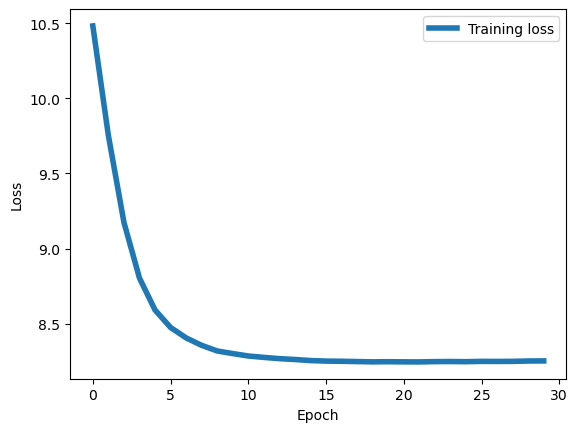
\includegraphics[width=0.5\textwidth]{loss_pro.png}
%     \label{fig:loss_pro}
%   }
%   \subfloat[Restruct specific spectra]
%   {
%     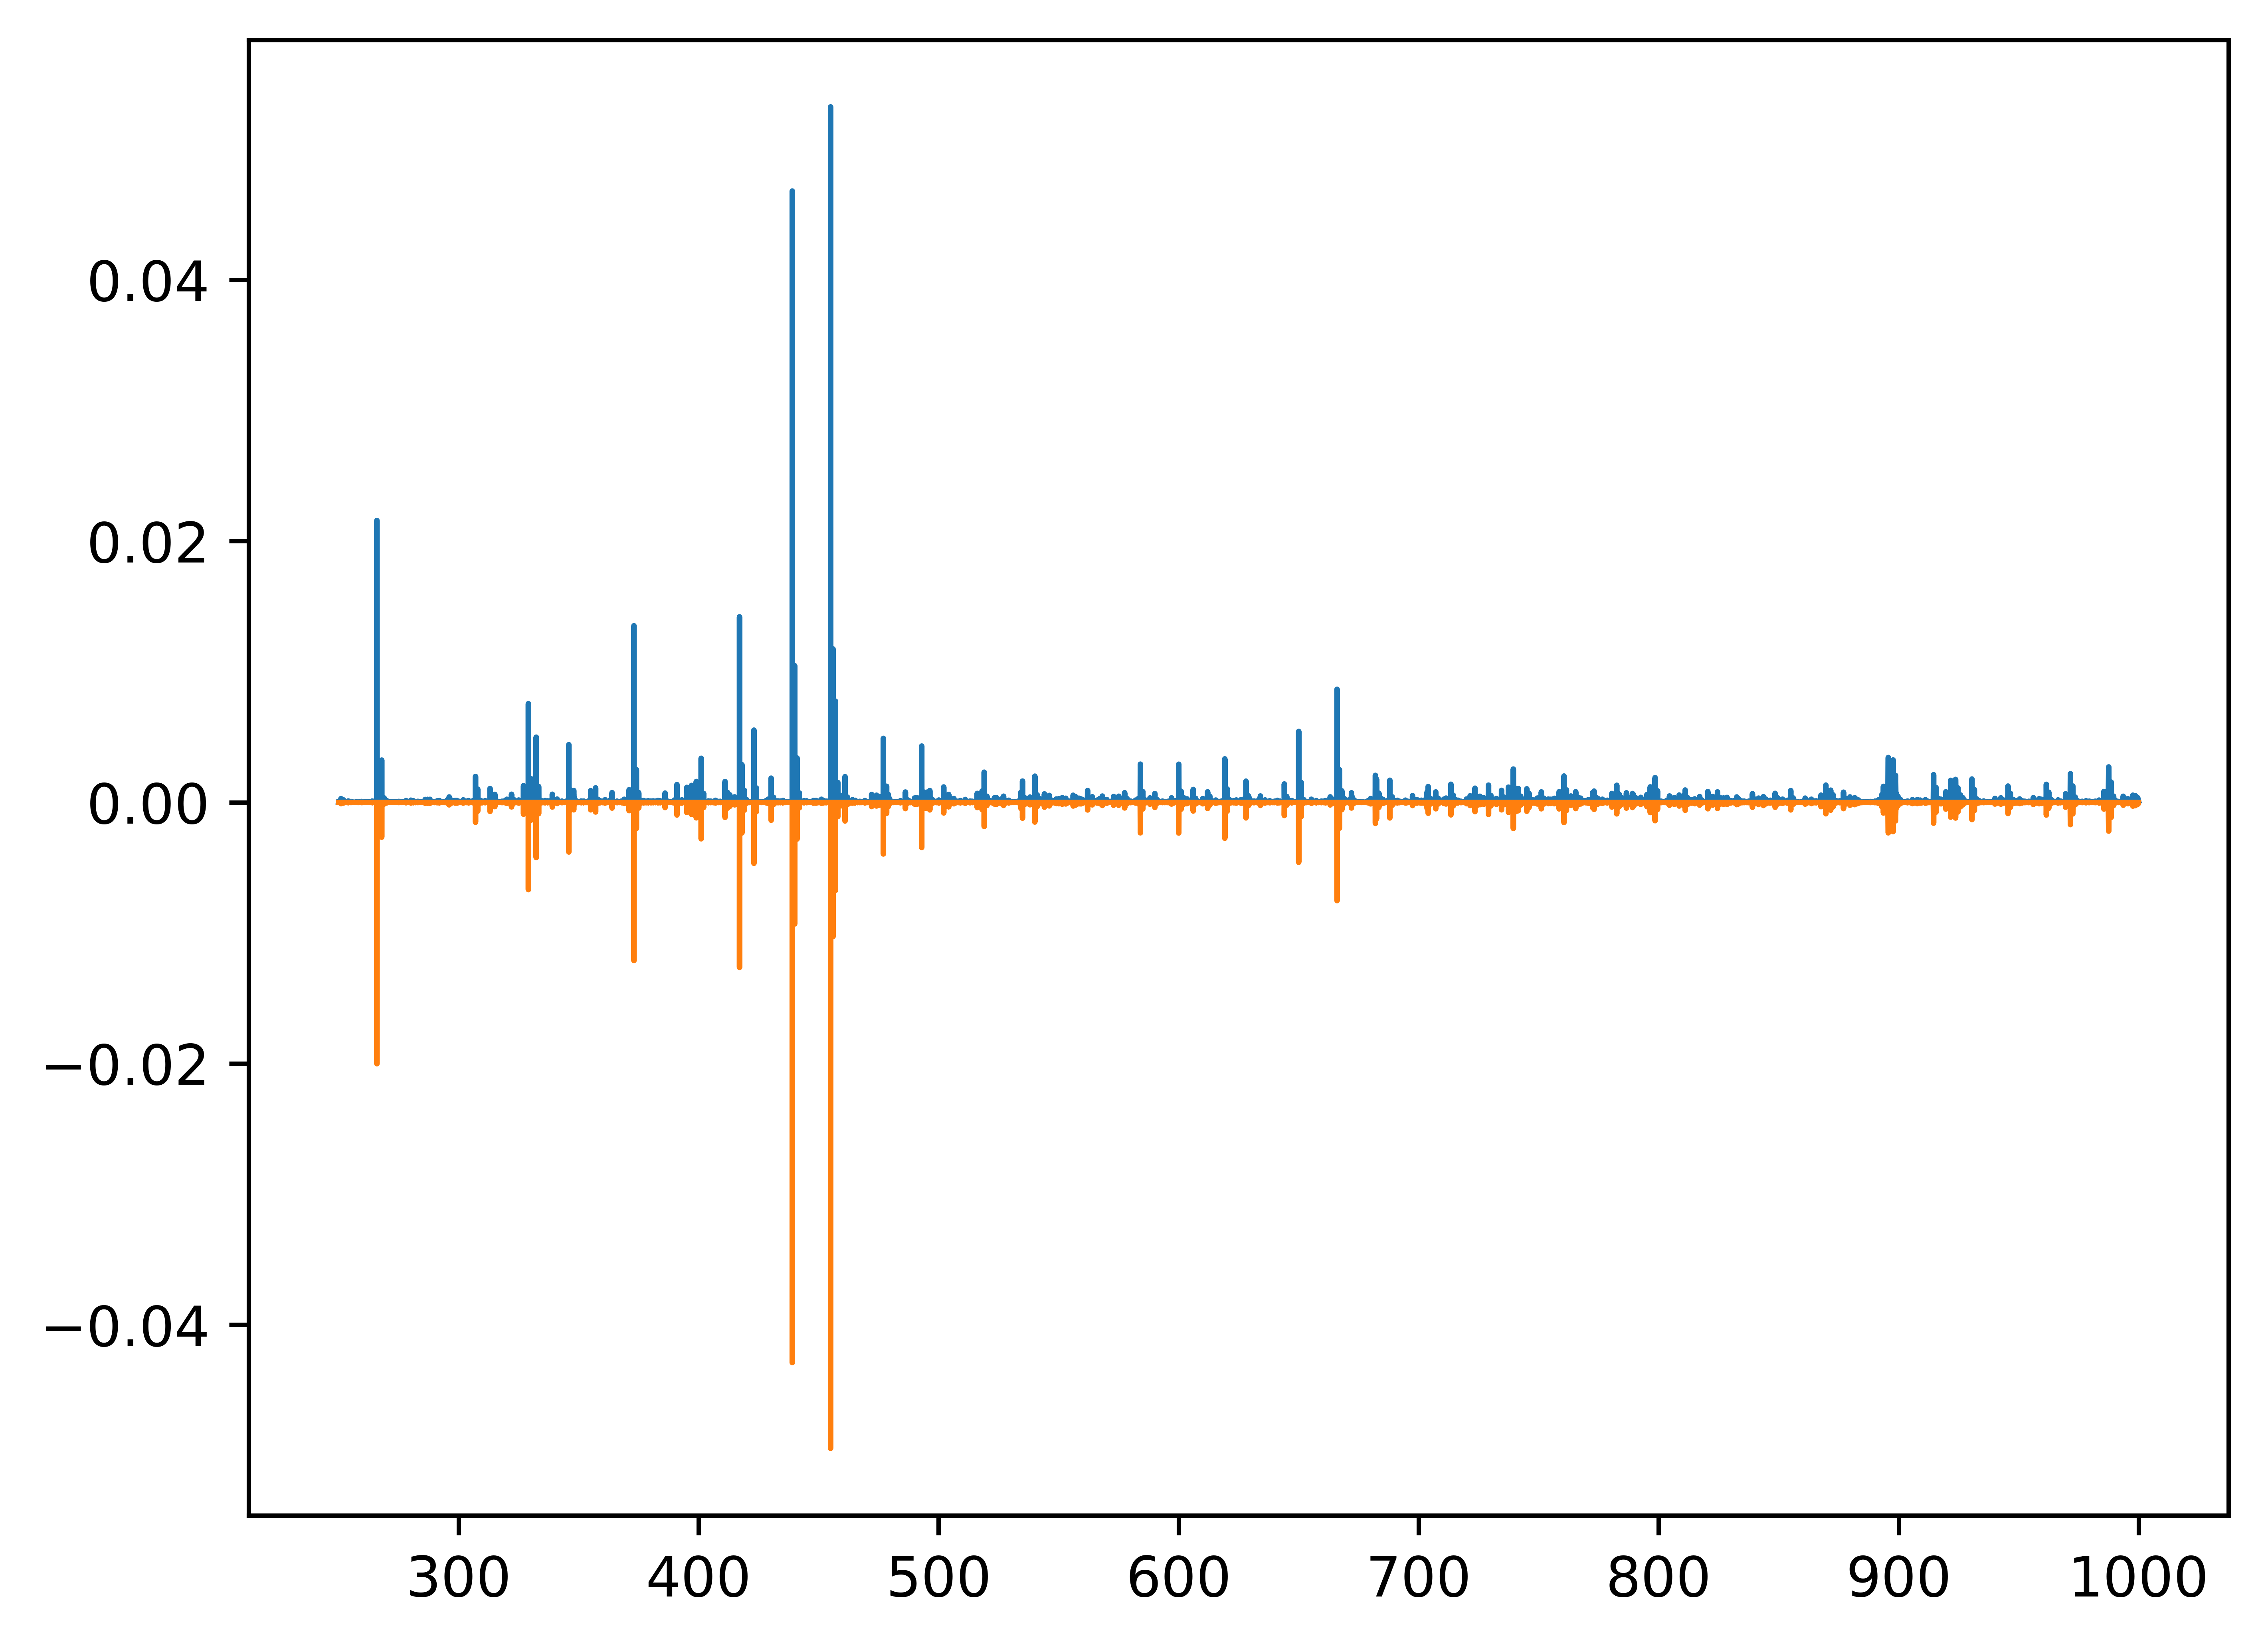
\includegraphics[width=0.5\textwidth,height=0.2\textheight]{pic/prostate/ori_pre.png}
%     \label{fig:spesific_restruct_train_pro}
%   }

%   \subfloat[clustering result]
%   {
%     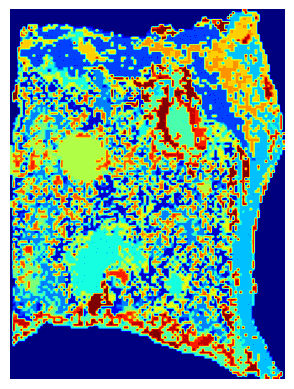
\includegraphics[width=0.2\textwidth]{./pic/prostate/clusters.png}
%     \label{fig:clusters_pro}
%   }
%   \subfloat[selected cluster]
%   {
%     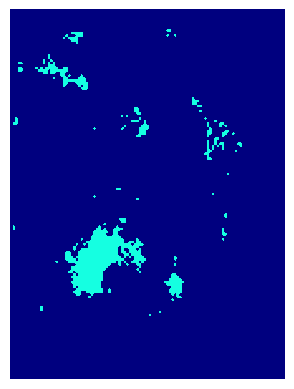
\includegraphics[width=0.2\textwidth]{./pic/prostate/selected.png}
%     \label{fig:selected_cluster_pro}
%   }  
%   \subfloat[selected m/z pattern]
%   {
%     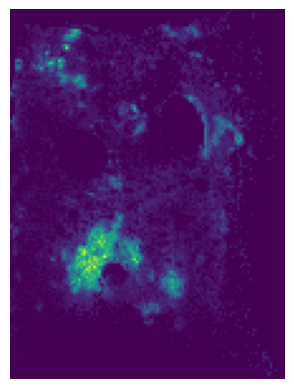
\includegraphics[width=0.2\textwidth]{./pic/prostate/selected_mz.png}
%     \label{fig:selected_mz_pro}
%   }  
%   \subfloat[histopathological annotation]
%   {
%     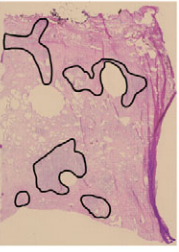
\includegraphics[width=0.185\textwidth]{./pic/prostate/op.png}
%     \label{fig:op_pro}
%   }
% \caption{Training phase}
% \label{fig:Training_pro}
% \end{figure} 


\begin{figure}[]
  \centering
  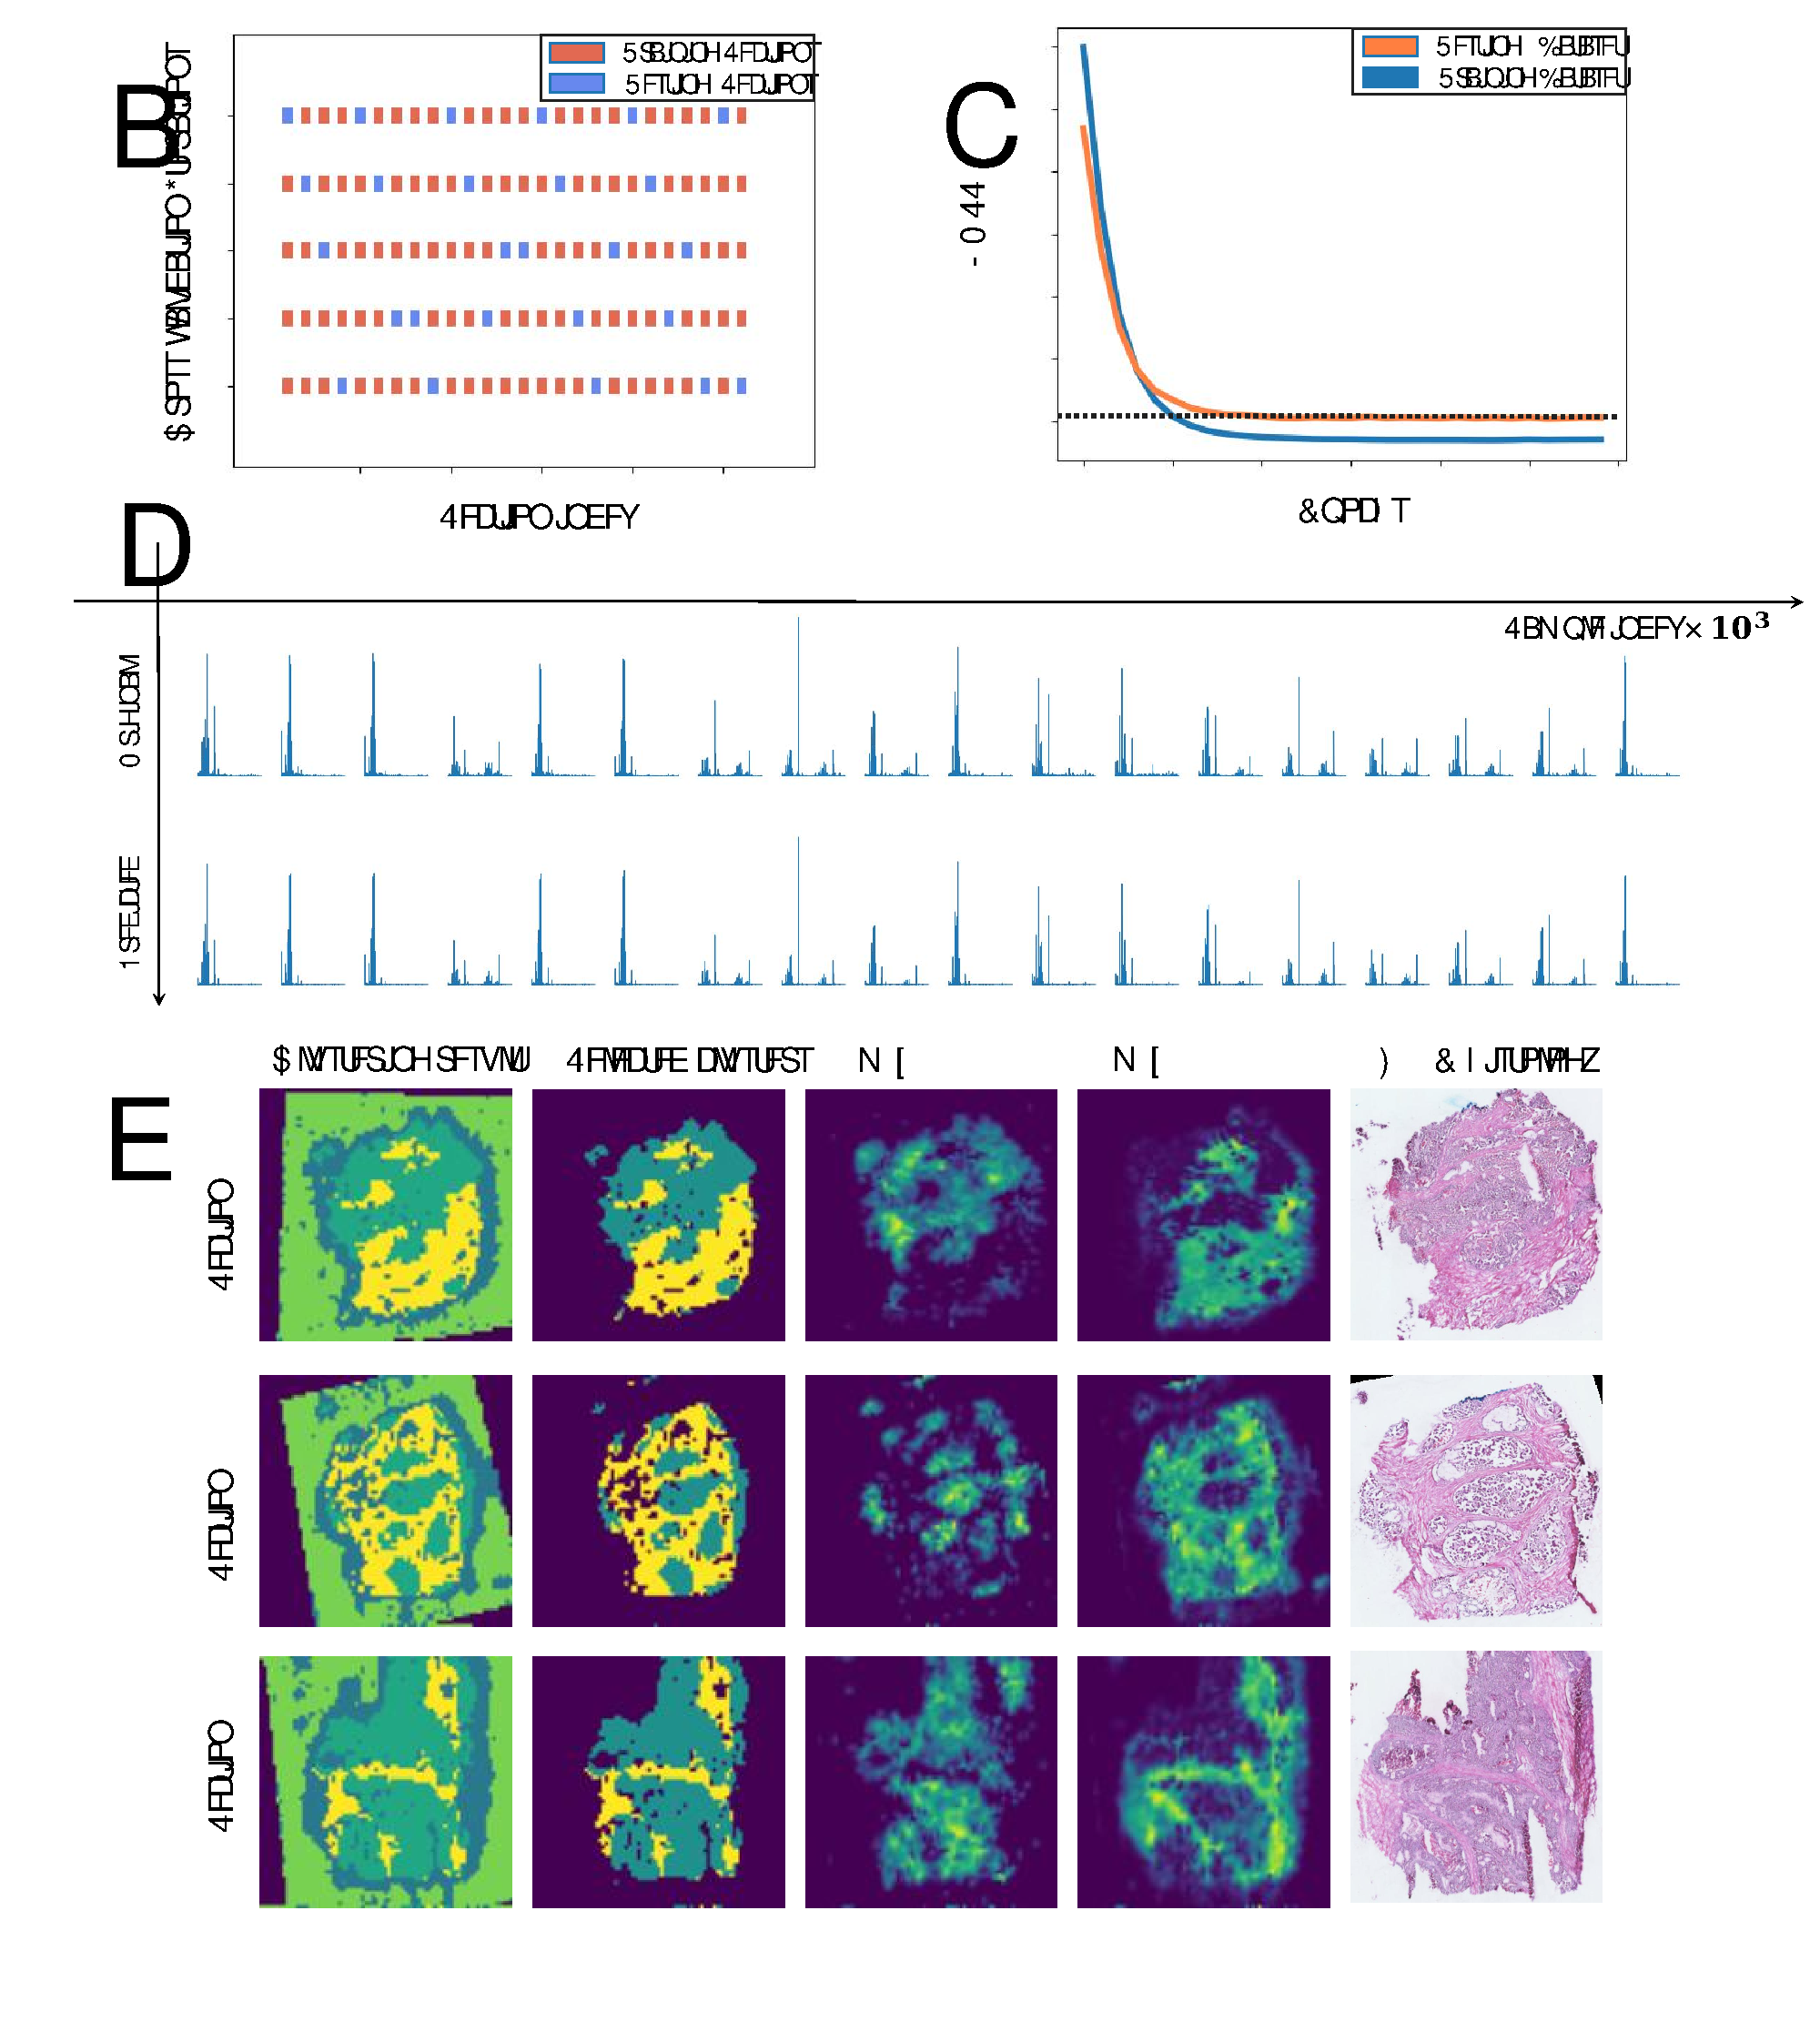
\includegraphics[width=\linewidth]{./pic/corlor_train.pdf}
\captionsetup{justification=raggedright,singlelinecheck=false}
\caption
  {
    \textbf{Analysis on colorectal carcinoma dataset (Training phase)}.  
    (a): 5-fold cross-validation analysis: The full MSI dataset is randomly shuffled and split 
    into an 80\% training set and a 20\% testing set, 
    and this procedure is iterated five times. 
    (b): The Atnal takes around 1.5 minutes to get convergence on the training set. 
    (93482 spectra each of 8073 dimensions). Here, the model with a moderate level of test error among the 5 models is selected for following performance analysis, which aims to obtain representative test results. 
    (c): Reconstruction results of some spectra. 
    (d): Those encoded features (Supplementary Figure \ref{fig:encoder_feature_3D_train}) 
    are clustered by the GMM, 
    and two clusters are selected  
    and found highly consistent with the cancerous and connective tissue in H\&E histology, respectively. 
    The intensities of two m/z channels (derived by correlation analysis) are found significantly raised in the area of these two clusters. 
  }
\label{fig:Training}
\end{figure}
\begin{figure}
  \centering
  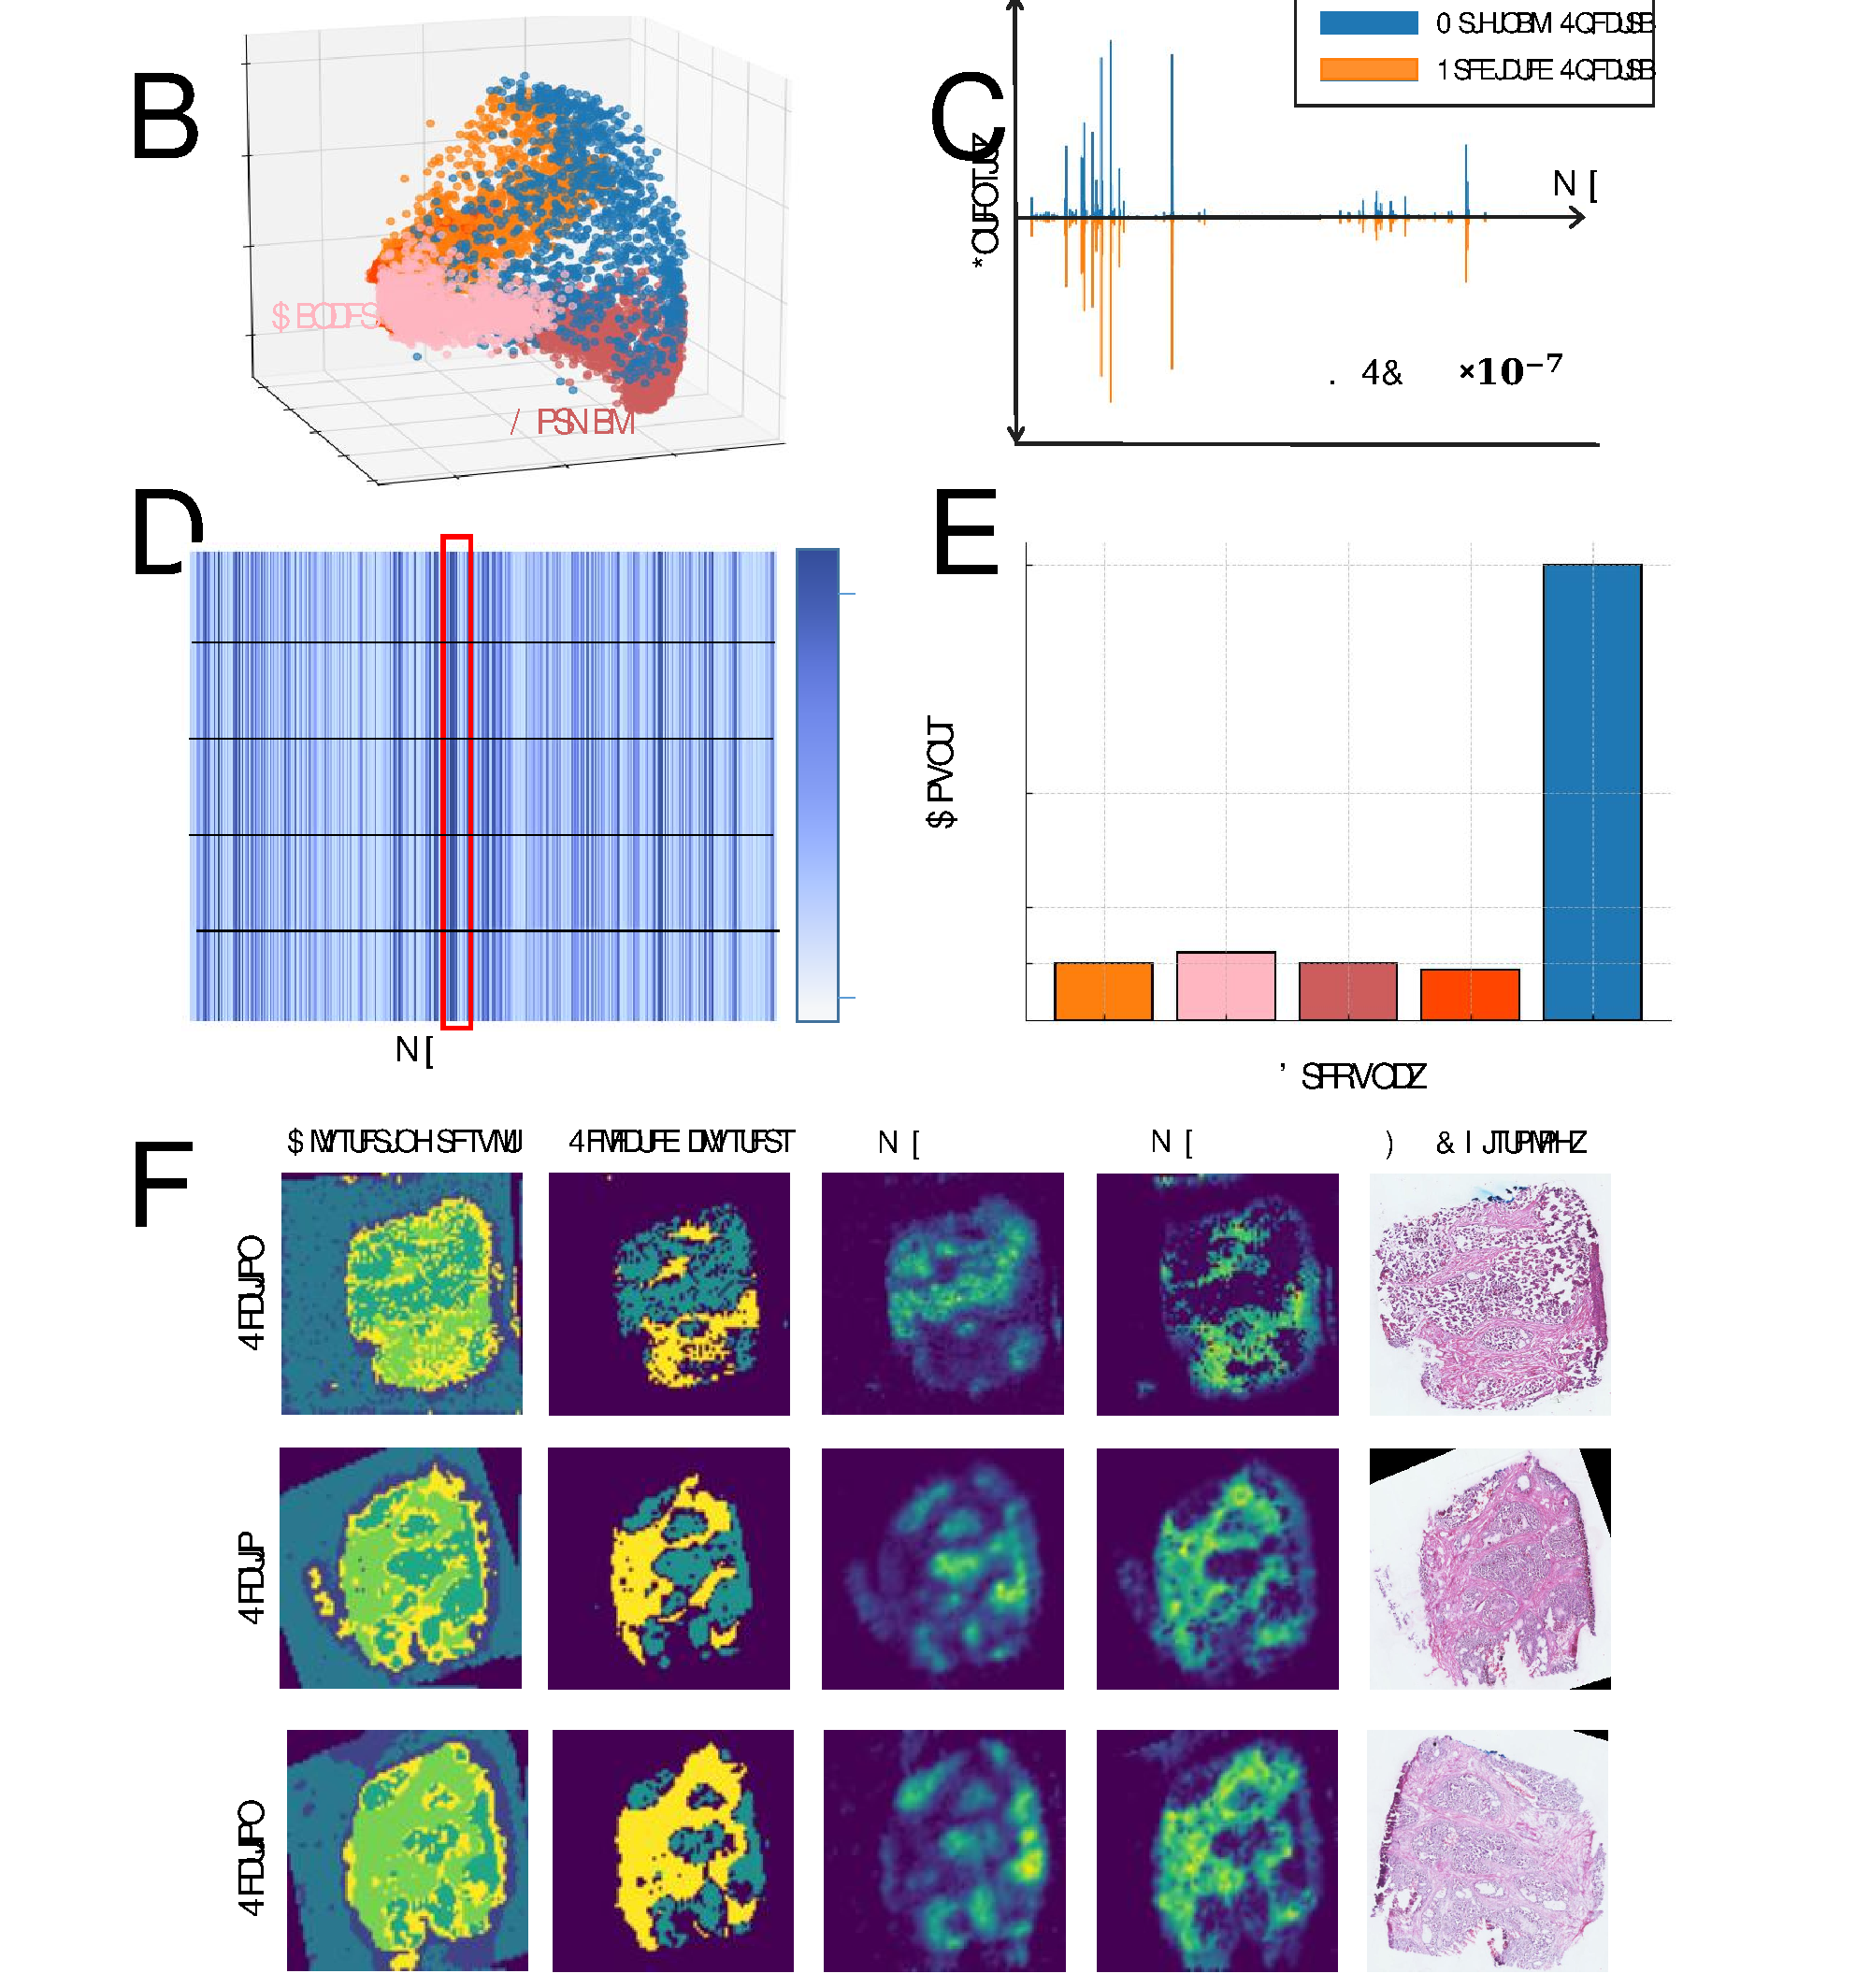
\includegraphics[width=\textwidth]{pic/color_test.pdf}
\captionsetup{justification=raggedright,singlelinecheck=false}
\caption
  {
    \textbf{Analysis of colorectal carcinoma dataset (Testing phase)}. 
    (a): The distribution of encoded features in a 3-dimensional space, which is reduced from 256 dimensions to a 3-dimensional space by using PCA for the purpose of visualization. 
    The spectra that respond to cancerous tissue 
    demonstrate spatial similarity, as do the spectra of normal (connective) tissue. These results in this phase are also derived from the moderate model as mentioned in the training phase. 
    (b): Average spectra of normalized original and 
    predicted data, with an overall reconstruction MSE of $2.1\times 10^{-7}$. 
    (c): In the five-fold cross-validation, 
    a heatmap is generated to depict the Pearson correlation coefficients between the 
    cancer cluster and all m/z channels. 
    (d): The statistical analysis encompasses all top 100 correlated m/z values 
    derived from the 5-fold cross-validation, yielding a total of 121 distinct values. 
    The majority of these values are consistently present across all 
    cross-validation iterations, demonstrating remarkable stability. 
    (e): Those encoded features (see Supplementary Figure \ref{fig:encoder_feature_3D_test}) 
    are clustered by the GMM, 
    and two clusters are selected.
    The selected clusters are found highly consistent 
    with the cancerous and connective tissue in H\&E histology, respectively. 
    Moreover, the intensities of two m/z channels (mentioned in the training phase) are also 
    found significantly raised in the area of these two clusters. 
  }



\label{fig:Testing}
\end{figure}

\begin{table}
  \centering
  \caption{\textbf{Identified compounds in the colorectal adenocarcinoma dataset}}
  \label{tbl:Compounds}
  \begin{tabular}{|c|p{15cm}|c|}
  \hline
  \textbf{M/Z Value} & \textbf{Identified Compounds}& \textbf{PPM} \\
  \hline
  720.495467
  &1-Myristoyl-2-adrenoyl-sn-glycero-3-phosphoethanolamine &1.87\\
  & 1-Oleoyl-2-a-linolenoyl-sn-glycero-3-phosphoethanolamine &1.87\\
  & 1-Arachidonoyl-2-palmitoyl-sn-glycero-3-phosphoethanolamine &1.87\\
  \hline
  858.5260627 
    & 1-(11Z,14Z-eicosadienoyl)-2-(4Z,7Z,10Z,13Z,16Z,19Z-docosahexaenoyl)-glycero-3-phosphoserine &3.49\\
   & 1-(5Z,8Z,11Z,14Z-eicosatetraenoyl)-2-(7Z,10Z,13Z,16Z-docosatetraenoyl)-glycero-3-phosphoserine &3.49\\
   & 1-(7Z,10Z,13Z,16Z-docosatetraenoyl)-2-(5Z,8Z,11Z,14Z-eicosatetraenoyl)-glycero-3-phosphoserine &3.49\\
   & 1-(4Z,7Z,10Z,13Z,16Z,19Z-docosahexaenoyl)-2-(11Z,14Z-eicosadienoyl)-glycero-3-phosphoserine &3.49\\
   % Add more rows as needed
  \hline 
  ...& For more details, please refer to Supplementary Table \ref{tab:colorectaltab-a},\ref{tab:colorectaltab-b} &...\\
  \hline
  \end{tabular}
\end{table}

\subsection{Analysis of the 3D DESI MSI data from colorectal adenocarcinoma dataset}
Here, we apply Atnal to reconstruct a 3D MSI volume from a human colorectal 
adenocarcinoma specimen: 26 consecutive 
(acquired at every 100 $\mu$m) 10 $\mu$m 
thickness tissue sections. 
To reduce the impact of imbalanced data splitting on model loss, 
we implement K-fold cross-validation during the process of the model 
training (Figure \ref{fig:Training}a), in which 26 tissue sections 
from the colorectal 
carcinoma specimen are divided into K groups. 
Each time one group is designated as the testing set, while the other 
groups are regarded as the training set. This is repeated K times, 
ensuring that each group can serve as the testing set at least once, and providing a 
comprehensive evaluation of model performance. 

In the MSI data of colorectal adenocarcinoma 
dataset, K is selected as 5 for the cross-validation. During 
each iteration of the 5-fold cross-validation, the data from 4 randomly selected groups, 
comprised of 20 tissue sections with a total of 93,482 spectra, 
are used to train Atnal. 
The training process of Atnal becomes convergent after approximately 15 epochs, 
as depicted in Figure \ref{fig:Training}b. The total running time cost for this 
convergence is approximately 1.5 minutes. Based on the encoded features 
(Supplementary Figure \ref{fig:encoder_feature_3D_train}) derived by 
the encoder of Atnal, the original spectra are 
reconstructed with an overall mean squared training error of $1.3 \times 10^{-7}$. For more training details, 
please refer to the accompanying figure \ref{fig:Training}c,\ref{fig:Training}d. 

Once the model training is completed, its performance is further evaluated by 
using the remaining 6 tissue sections with 29,006 spectra (testing set).
The spectra in the same batch 
are loaded into the memory and analyzed by Atnal. 
It takes approximately 4 s for the encoder of Atnal 
to predict the encoded features and another 3 s for the decoder 
to reconstruct the data. 
The strong resemblance observed between the original and reconstructed spectra, 
as shown in Figure \ref{fig:Testing}b, indicates that the encoder 
successfully captures the intricate features present in the nonlinear 
manifold of the original high-dimensional data. 

The encoded features, in Supplementary Figure \ref{fig:encoder_feature_3D_test}, represent a 
256-dimensional nonlinear embedding of the original high-dimensional testing data. 
The overall mean square testing error between the reconstructed and original data
is  $2.1 \times 10^{-7}$. 
The testing results, 5 GMM clusters, of the encoded features, carry significant 
implication: 2 of 5 GMM clusters associate with tumor and connective tissue. 
This implication is consistent with the results of previous studies 
\cite{abdelmoula2018interactive} \cite{oetjen2015benchmark} 
and images of the H\&E stained tissue sections,  see 
Figure \ref{fig:Testing}e (H\&E histology)   
and Supplementary Figure \ref{fig:op of colorectal adenocarcinoma dataset}. 

The encoded features are then clustered by GMM (K = 5), forming five clusters, 
and two of them (cluster 3 and cluster 5) show
a high degree of consistency with 
histological evaluation (H\&E) as illustrated  
in Figure \ref{fig:Testing}e (H\&E histology) and  
Supplementary Figure \ref{fig:Clusters of colorectal adenocarcinoma dataset}. 
These two clusters correlate with 
the ions at m/z 720.4954
(Supplementary Figure \ref{fig:tumor colorectal adenocarcinoma dataset}) 
and m/z 766.53, of which the  Pearson correlation 
values are 0.7761 and 0.746, respectively.
Moreover, this result is consistent with the observation that 
the intensities of the ions at m/z 720.49 and m/z 766.53 are 
particularly high in tumor and connective tissue, respectively. 
 
% \begin{figure}[htbp]
%   \centering
%   \begin{minipage}[c]{0.44\textwidth}
%     % \flushleft 
%     \subfloat[Training/Testing set split]
%     {
%       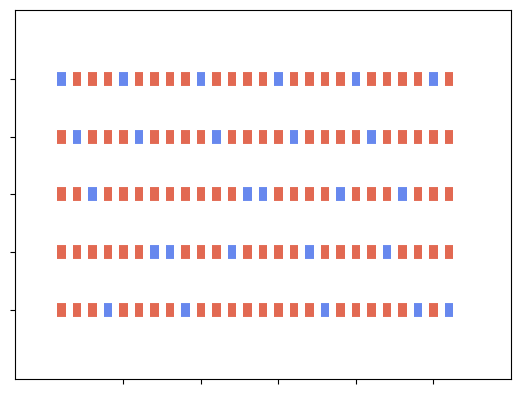
\includegraphics[width=0.94\textwidth]{k_fold.png}
%       \label{fig:k_fold}
%     }\\
%     \vspace{-5pt}
%     \subfloat[Traing loss]
%     {
%       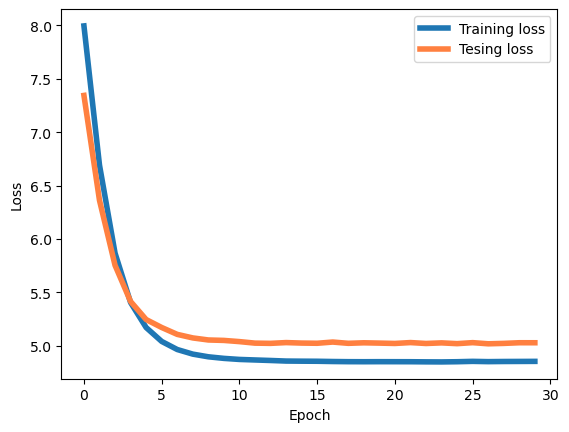
\includegraphics[width=0.77\textwidth]{loss.png}
%       \label{fig:loss}
%     }
%   \end{minipage}
%   \hfill
  
%   \subfloat[Restruct specific spectra]
%   {
%     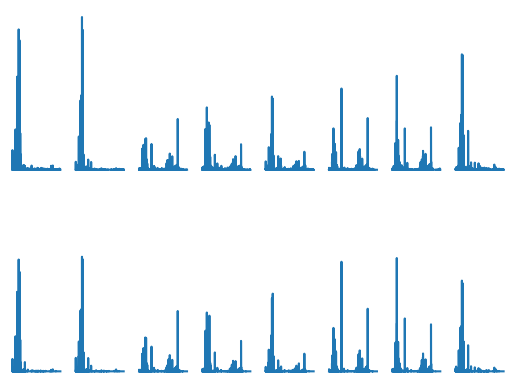
\includegraphics[width=0.5\textwidth,height=0.2\textheight]{spesific_restruct_train.png}
%     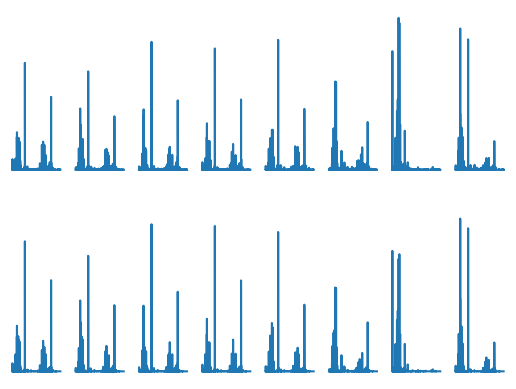
\includegraphics[width=0.5\textwidth,height=0.2\textheight]{spesific_restruct_test.png}
%     \label{fig:spesific_restruct_train}
%   }

%   \subfloat[Section4]
%   {
%     
\includegraphics[width=0.2\textwidth,height=0.137\textheight]{../Results_CV/Section3/clusters .png}
%     
\includegraphics[width=0.2\textwidth,height=0.137\textheight]{../Results_CV/Section3/cluster35.png}
%     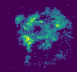
\includegraphics[width=0.2\textwidth,height=0.137\textheight]{../Results_CV/Section3/cluster3.png}
%     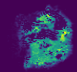
\includegraphics[width=0.2\textwidth,height=0.137\textheight]{../Results_CV/Section3/cluster5.png}
%     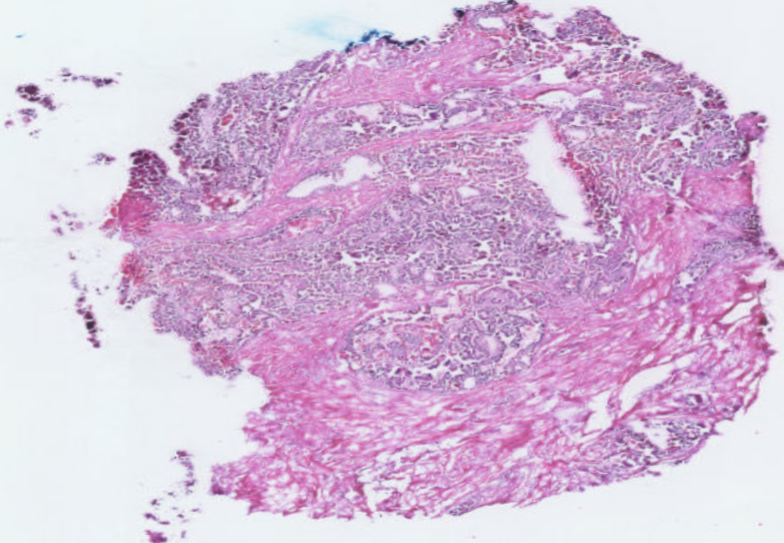
\includegraphics[width=0.2\textwidth,height=0.137\textheight]{../Results_CV/Section3/op.png}
%     \label{fig:clustering_4}
%   }
%   % \subfloat[Section9]
%   % {
%   %   
\includegraphics[width=0.2\textwidth,height=0.137\textheight]{../Results_CV/Section8/clusters .png}
%   %   
\includegraphics[width=0.2\textwidth,height=0.137\textheight]{../Results_CV/Section8/cluster35.png}
%   %   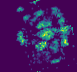
\includegraphics[width=0.2\textwidth,height=0.137\textheight]{../Results_CV/Section8/cluster3.png}
%   %   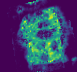
\includegraphics[width=0.2\textwidth,height=0.137\textheight]{../Results_CV/Section8/cluster5.png}
%   %   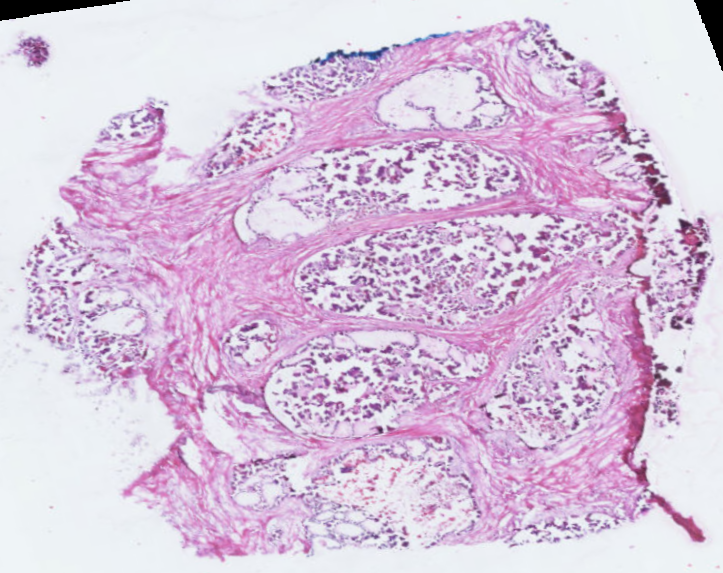
\includegraphics[width=0.2\textwidth,height=0.137\textheight]{../Results_CV/Section8/op.png}
%   %   \label{fig:clustering_9} 
%   % }

%   % \subfloat[Section26]
%   % {
%   %   
\includegraphics[width=0.2\textwidth,height=0.137\textheight]{../Results_CV/Section25/clusters .png}
%   %   
\includegraphics[width=0.2\textwidth,height=0.137\textheight]{../Results_CV/Section25/cluster35.png}
%   %   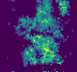
\includegraphics[width=0.2\textwidth,height=0.137\textheight]{../Results_CV/Section25/cluster3.png}
%   %   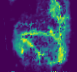
\includegraphics[width=0.2\textwidth,height=0.137\textheight]{../Results_CV/Section25/cluster5.png}
%   %   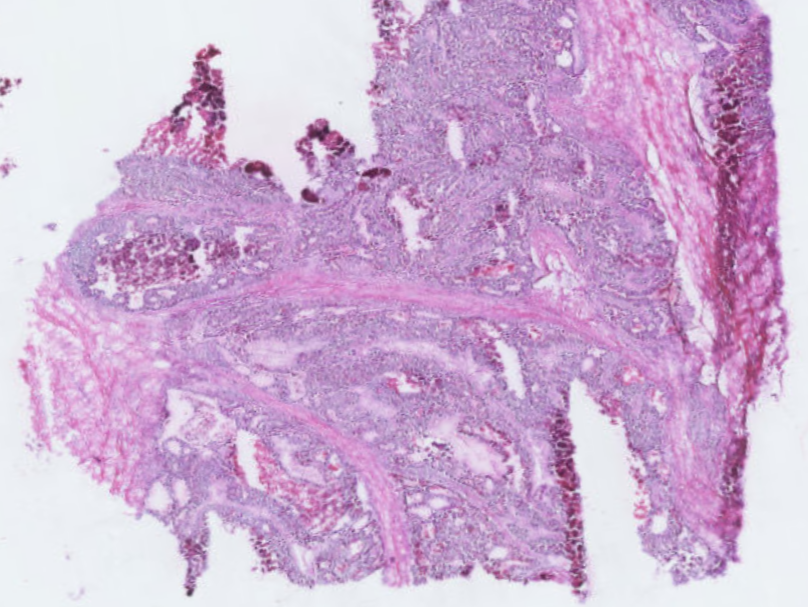
\includegraphics[width=0.2\textwidth,height=0.137\textheight]{../Results_CV/Section25/op.png}
%   %   \label{fig:clustering_26} 
%   % }
% \caption{Training phase}
% \label{fig:Training}
% \end{figure}


14 m/z values are discovered to be 
strongly correlated with colorectal carcinoma. 
As checked with the Human Metabolome Database (HMDB), 
the LIPID MAPS® Structure Database (LMSD) 
and MetaboAnalyst database, 
9 out of 14 are successfully identified. For instance, m/z 858.5260627 
is identified as compounds belonging to the class of phosphatidylserines 
with a  tolerance window of 5 ppm, as shown in Table \ref{tbl:Compounds}. 
They are speculated to be related 
to the vigorous phospholipid metabolism of colorectal cancer cells. Nevertheless, 
there is no relevant report on phosphatidylserine compounds as colorectal cancer markers. 
For more details on the identification of these compounds, 
see Supplementary Table \ref{tab:colorectaltab-a},\ref{tab:colorectaltab-b}.

% \begin{figure}[htbp]
%   \centering
%   \subfloat[Encoded features in testing set]
%     {
%       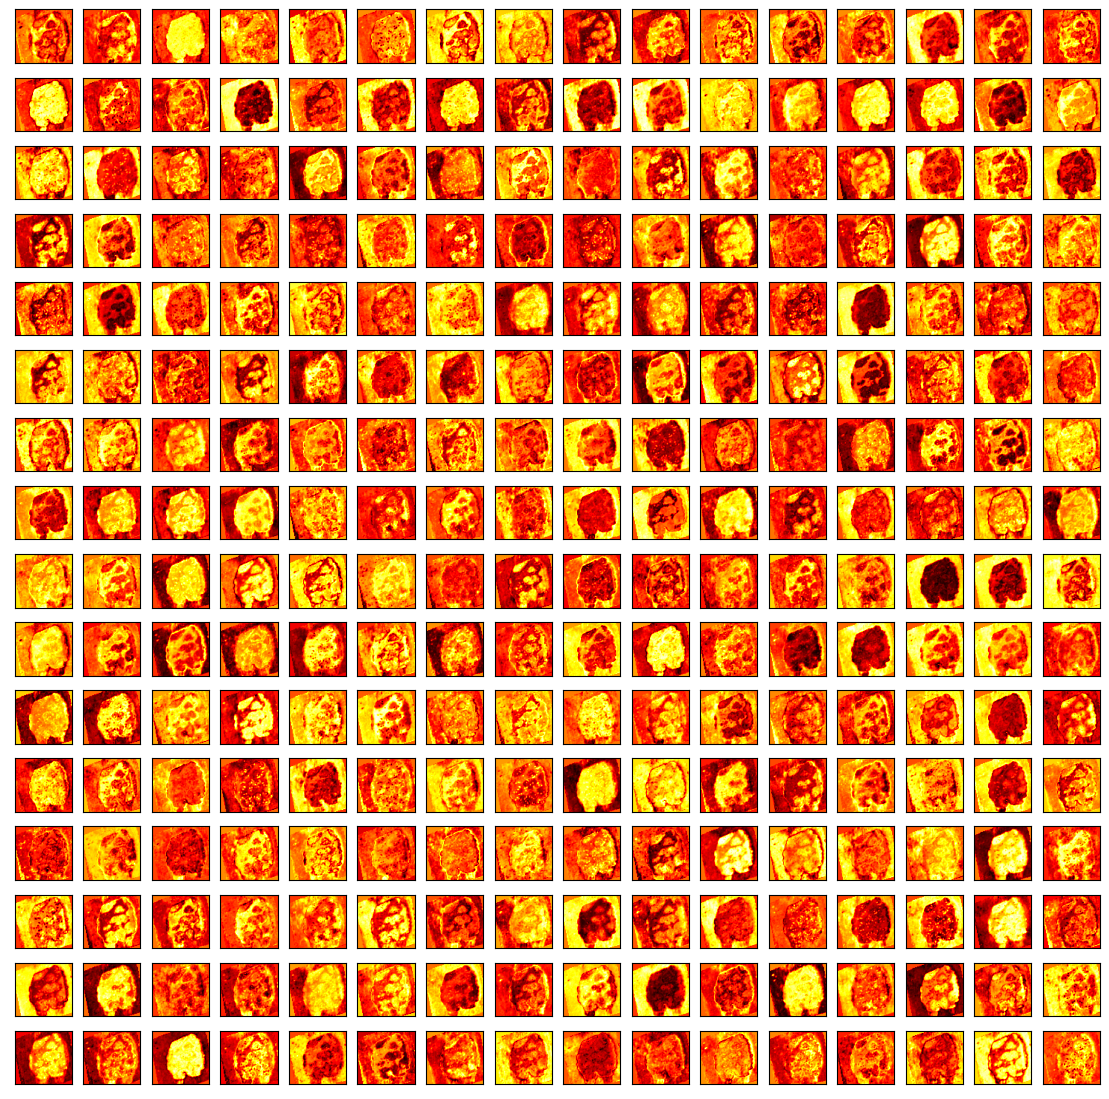
\includegraphics[width=0.32\textwidth]{pic/encoder_feature_3D_test.png}
%       \label{fig:encoder_feature_3D_test}
%     }
%     \subfloat[scatter]
%     {
%       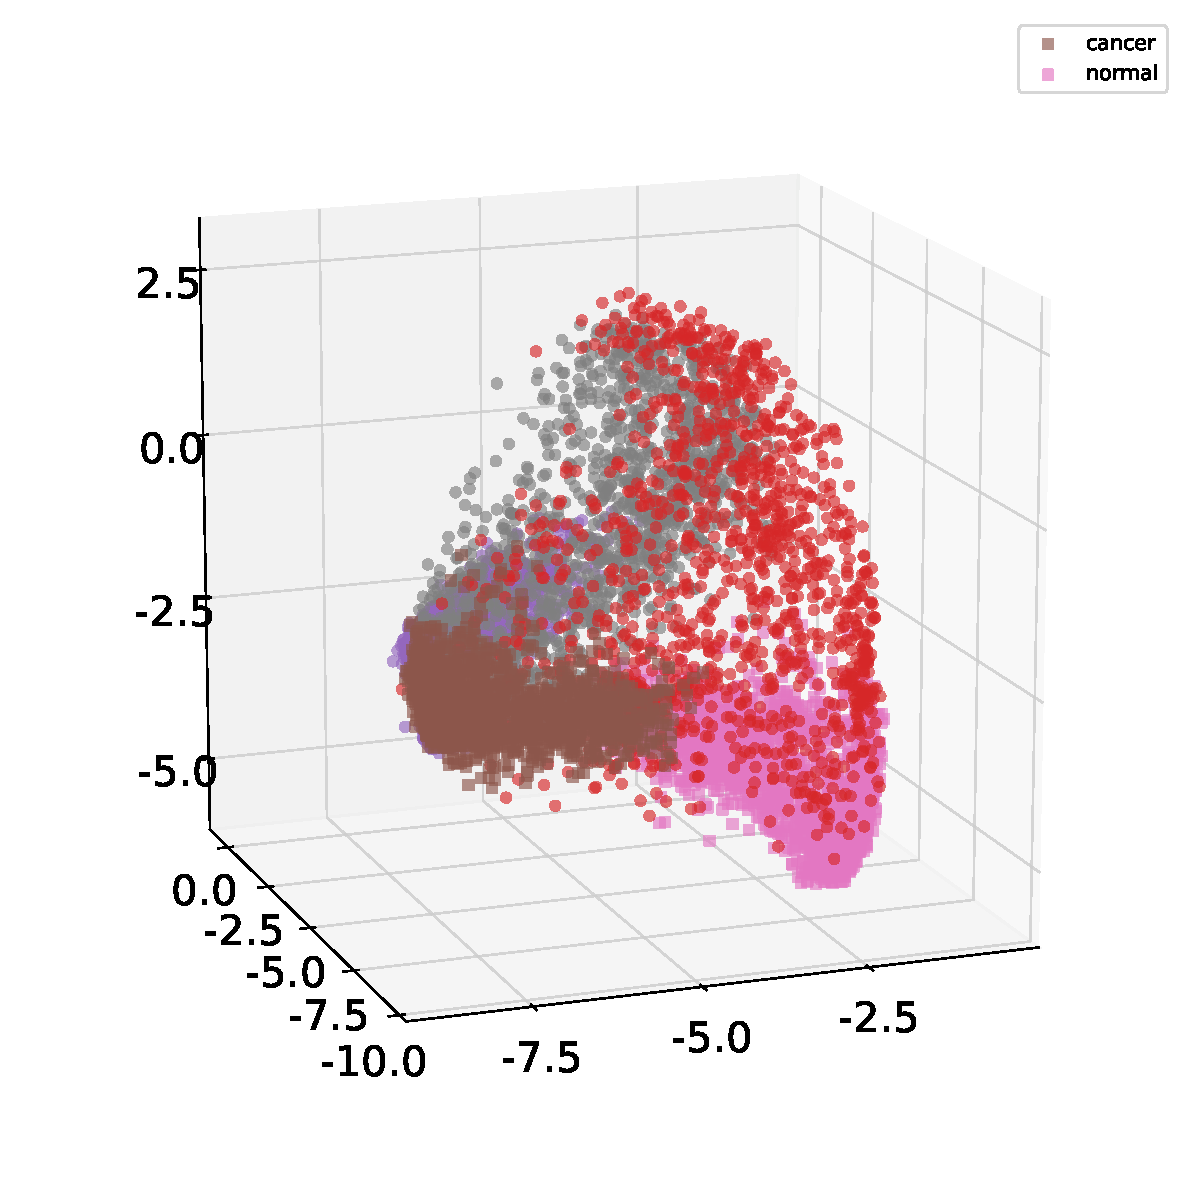
\includegraphics[width=0.6\textwidth]{pic/colorectal/scatter.pdf}
%       \label{fig:scatter}
%     }
%     \\
%   \subfloat[Section 1]
%   {
%     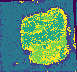
\includegraphics[width=0.2\textwidth,height=0.137\textheight]{../Results_CV/Section0/clusters .png}
%     
\includegraphics[width=0.2\textwidth,height=0.137\textheight]{../Results_CV/Section0/cluster34.png}
%     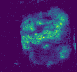
\includegraphics[width=0.2\textwidth,height=0.137\textheight]{../Results_CV/Section0/cluster3.png}
%     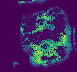
\includegraphics[width=0.2\textwidth,height=0.137\textheight]{../Results_CV/Section0/cluster4.png}
%     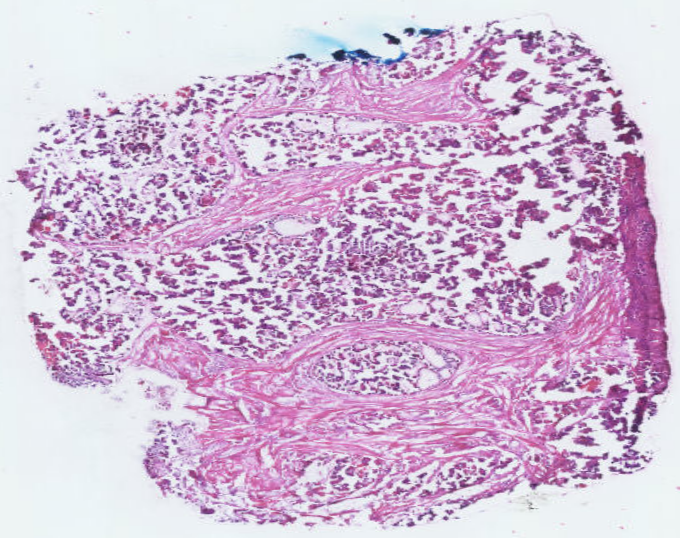
\includegraphics[width=0.2\textwidth,height=0.137\textheight]{../Results_CV/Section0/op.png}
%     \label{fig:clustering_1}
%   }

%   \subfloat[Section 11]
%   {
%     
\includegraphics[width=0.2\textwidth,height=0.137\textheight]{../Results_CV/Section10/clusters .png}
%     
\includegraphics[width=0.2\textwidth,height=0.137\textheight]{../Results_CV/Section10/cluster34.png}
%     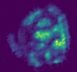
\includegraphics[width=0.2\textwidth,height=0.137\textheight]{../Results_CV/Section10/cluster3.png}
%     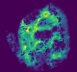
\includegraphics[width=0.2\textwidth,height=0.137\textheight]{../Results_CV/Section10/cluster4.png}
%     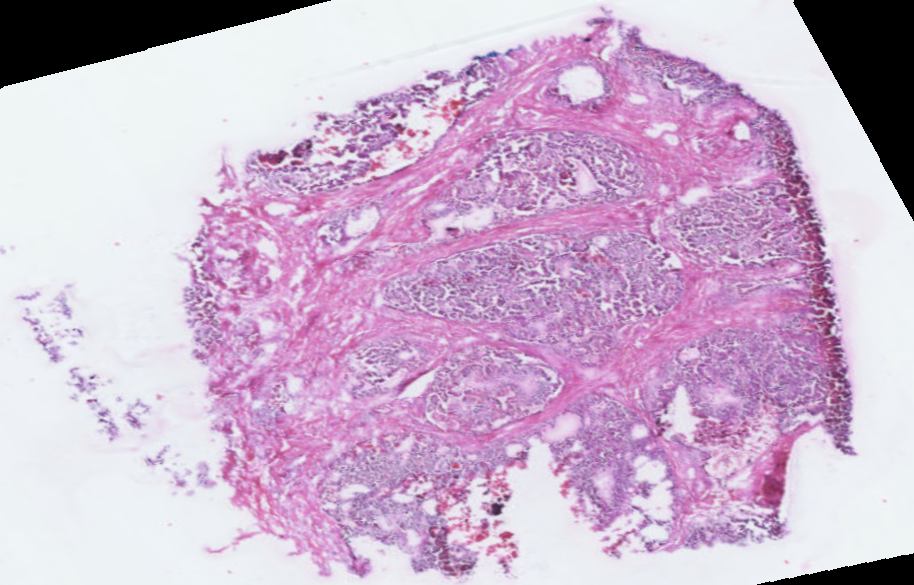
\includegraphics[width=0.2\textwidth,height=0.137\textheight]{../Results_CV/Section10/op.png}
%     \label{fig:clustering_11}
%   }

%   \subfloat[Section 13]
%   {
%     
\includegraphics[width=0.2\textwidth,height=0.137\textheight]{../Results_CV/Section12/clusters .png}
%     
\includegraphics[width=0.2\textwidth,height=0.137\textheight]{../Results_CV/Section12/cluster34.png}
%     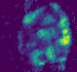
\includegraphics[width=0.2\textwidth,height=0.137\textheight]{../Results_CV/Section12/cluster3.png}
%     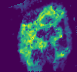
\includegraphics[width=0.2\textwidth,height=0.137\textheight]{../Results_CV/Section12/cluster4.png}
%     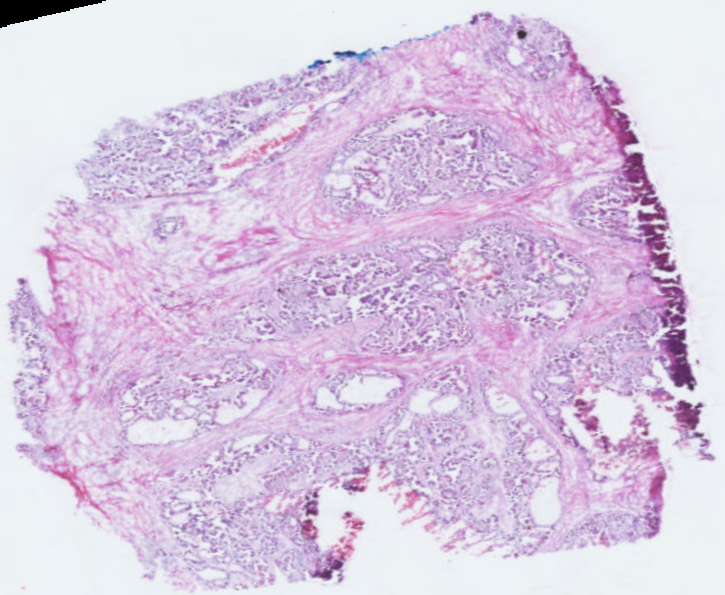
\includegraphics[width=0.2\textwidth,height=0.137\textheight]{../Results_CV/Section12/op.png}
%     \label{fig:clustering_13}
%   }
% \caption{Testing phase}
% \label{fig:Testing}
% \end{figure}  


  
 
\subsection{Discussion}
In this study, a novel method called Atnal is developed 
for analyzing MSI data collected from different types of 
human tissue. It can be used to reveal heterogeneity in cancer 
tissue, discover  
cancer biomarkers, and assist in cancer clinical diagnosis.
In the following, we discuss the details of the training and application 
(dimension reduction, clustering and correlation analysis) of Atnal. 
% \begin{figure}[htbp]
%   \centering
%   \begin{minipage}{0.46\textwidth}
%     \subfloat[Pearson in msiPL and Atnal]{
%       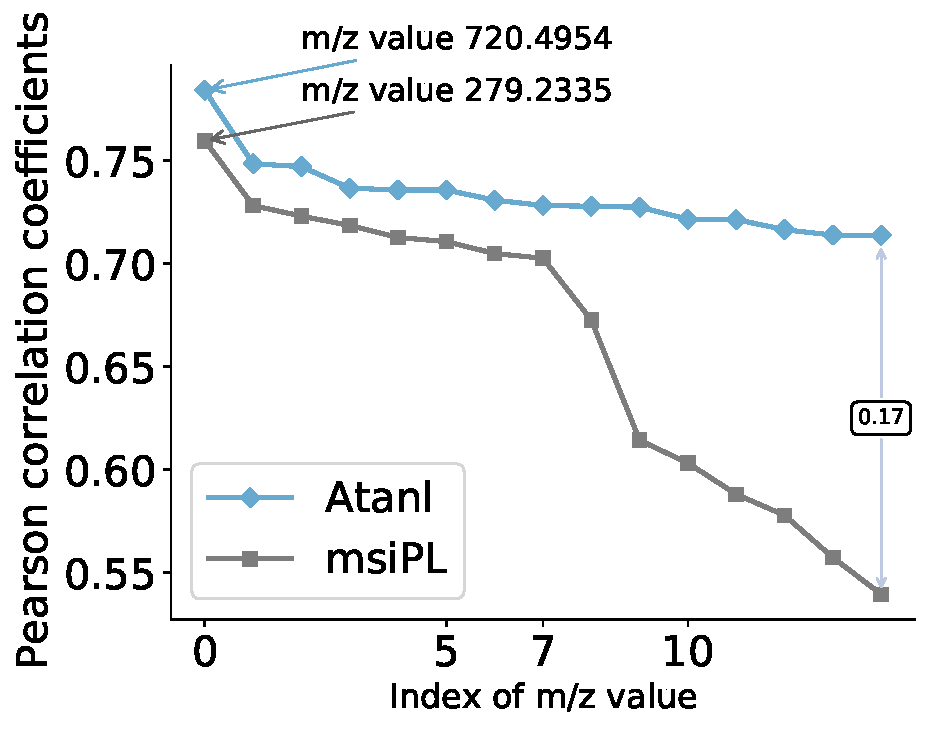
\includegraphics[width=\textwidth]{pic/pearson.pdf}
%     }
%   \end{minipage}
%   \begin{minipage}{0.51\textwidth}
%     \subfloat[Loss of different models]
%     {
%     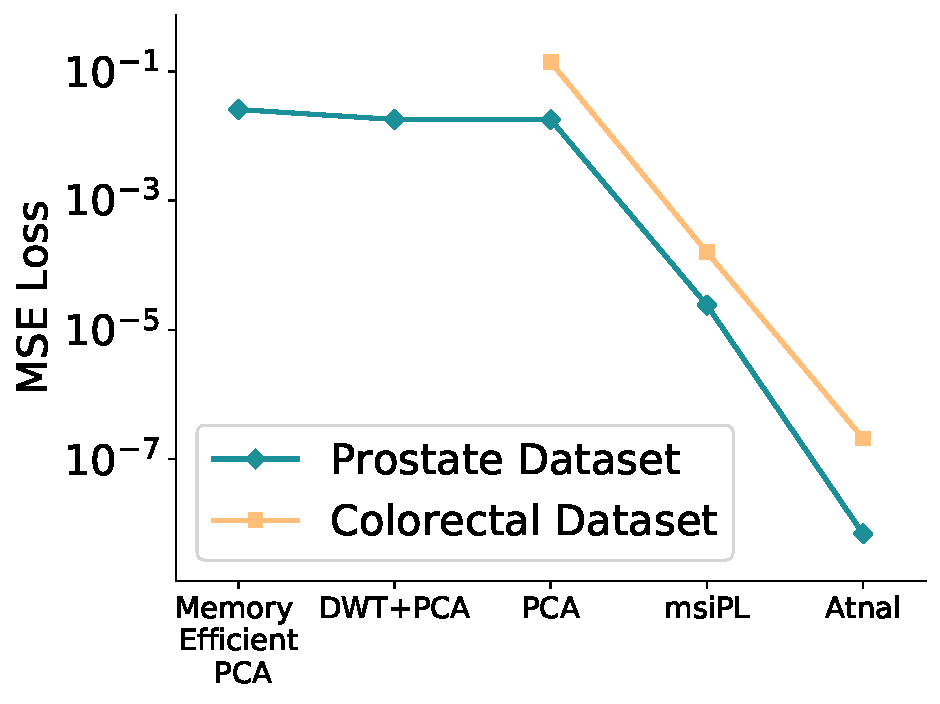
\includegraphics[width=\textwidth]{pic/loss.pdf}
%     }
%   \end{minipage}
% \caption{Quantitative comparative analysis of model performance}
% \label{fig:model performance}
% \end{figure}
\begin{figure}[htbp]
  \centering
  \includegraphics[width=0.8\linewidth]{pic/result.pdf}
\captionsetup{justification=raggedright,singlelinecheck=false}
\caption
  { 
    \textbf{Quantitative comparative analysis of model performance}. 
  (a): The m/z values identified by Atnal exhibit significantly higher 
  correlations with cancerous regions compared to those found by msiPL, 
  as observed in the dataset of colorectal adenocarcinoma. Moreover, 
  Atnal effectively circumvents the omission of crucial m/z values. 
  (b): The loss (log(MSE)) between original and reconstructed 
  MSI data computed via  
  various techniques. 
  Results on the prostate cancer dataset reflect the training errors, while the 
  results on the colorectal carcinoma dataset represent the testing errors.  
  Even when contrasted with the latest method 
  msiPL, Atnal demonstrates an error 
  reduction of at least two orders of magnitude 
  across both prostate cancer and colorectal adenocarcinoma datasets. 
  }
\label{fig:model performance}
\end{figure}
\begin{table}[htbp]
  \centering
  \caption{\textbf{MSEs for MSI data reconstruction}}
  \label{tbl:model performance}
  \begin{tabular}{cccc}
    \toprule
    & \textbf{PCA} & \textbf{msiPL} & \textbf{Atnal} \\
    \midrule
    \textbf{MSI Prostate Dataset} & $1.8 \times 10^{-2}$ & $6.9 \times 10^{-5}$ & $7.0 \times 10^{-9}$ \\
    \textbf{MSI Colorectal carcinoma Dataset} & $1.4 \times 10^{-1}$ & $1.6 \times 10^{-4}$ & $2.1 \times 10^{-7}$ \\
    \bottomrule
  \end{tabular}
\end{table}
\begin{table}[htbp]
  \centering
  \caption{\textbf{Ablation of Atnal with colorectal carcinoma dataset}}
  \label{tab:ablation_experiment}
  \begin{tabular}{ccc}
    \toprule
    & \multicolumn{2}{c}{\textbf{Loss}} \\
    \cmidrule{2-3}
    \textbf{Experimental Condition} & \textbf{Training} & \textbf{Testing} \\
    \midrule
    \textbf{Base} & $1.567 \times 10^{-7}$ & $2.262 \times 10^{-7}$ \\
    \textbf{Base + Residual} & $2.02 \times 10^{-7}$ & $2.86 \times 10^{-7}$ \\
    \textbf{Base + Attention} & $4.2 \times 10^{-7}$ & $8.1 \times 10^{-7}$ \\
    \textbf{Base + Attention + Residual} & $\mathbf{1.41 \times 10^{-7}}$ & $\mathbf{2.119 \times 10^{-7}}$ \\
    \bottomrule
  \end{tabular}
\end{table}


\textbf{Training}: During the training, self-supervised learning is employed to extract prior 
information from the raw data; 
ReLU activation functions are extensively 
adopted to introduce non-linearity; and Softmax 
activation functions are used  in the final output layer to 
ensure the reconstructed data values have the same range as the  
normalized input, that is, from 0 to 1. 
The consistency of the value range between the input and output layers is 
crucial for minimizing the loss function expressed 
by Equation \ref{eqn:loss function}. 
Adopting the learning rate decay in self-supervised learning,
Atnal shows strong generalization and excellent performance on 
reconstructing original data, and avoids overfitting
the training data, as shown in Figure \ref{fig:Training}b. 
Without manual feature 
engineering during mass spectrometry 
imaging data analysis, Atnal can accelerate the identification of 
biologically relevant ions and reduce the biases introduced 
by subjective factors, thereby promoting the process of 
biomarker discovery. 
The loss function is given by 
the categorical cross-entropy that assigns higher weights 
to non-zero data in the spectral data 
and makes Atnal more sensitive to the reconstruction of the original data. 
Atnal uses mini-batch training, which allows 
loading only a small portion of the spectral 
data into the graphics memory. This enables the Graphics Processing Units (GPUs) to process
large and complex datasets, and empowers Atnal to 
conduct single-precision floating-point training on a workstation 
with 64 GB of memory and 8 GB of graphics memory. 


As the kernel of Atnal, the attention mechanism simulates the human 
attention mechanism, and assists Atnal in focusing on 
relevant parts of the input sequence 
in the spectra by treating 
the intensity  
at different m/z values as the features of these spectra. Without any 
positional information, the attention 
matrices between different spectra are  constructed  to discover the 
intrinsic correlations among these spectra. 
In the Attention Block ($h_3$), the keys, values, and queries (mentioned 
in Equation \ref{eqn:MultiHeadAttn}) are all derived 
from the output of the previous layer $MLP_e$ ($h_2$) in the encoder. 
As a normal module used in deep neural networks, the residual connection module 
provides a direct flow of information inner $h_3$. 
To test the functions of the 
attention module and the residual connection module, 
we conduct an ablation experiment. 
As shown in Table \ref{tab:ablation_experiment}, 
using only one of the two modules results in a varying degree of 
decrease in model performance. 
Moreover, as a comparison, when we incorporate both the attention module and the 
residual connection module as submodules in Atnal, we can 
achieve optimal results.

Now we analyze the reasons for the experiment result above. 
The attention module enables the model to learn the 
weights of different positions in the input, and allows for 
focusing on the spectra located in the positions with high weights 
and reducing the interference from the information with low weights. 
But, relying only 
on the attention module (without residual module) may lead 
to an excessive attention on some certain 
positions or features.
Similarly, the residual connection module may facilitate direct information 
propagation within networks and respond to challenges from the  gradient 
vanishing and exploding, so as to reduce information loss in deep 
networks on one hand. On the other hand, only using the residual 
connection module may introduce 
too much information flow, which results in an overreliance on previous 
layers and limits model stability and expressive capacity. 
As seen, integrating the residual connection module and the attention module 
contribute to a balance between these advantages and disadvantages, which benefits  
both the information transmission and selection, 
thus enhancing the overall performance.

% As for the learnable parameters of Atnal, their scale is huge: 
% 11.17 million, which makes Atnal a large model. Nonetheless, Atnal can be easily 
% trained. Specificly, Atnal converges in only 10 epochs, and it only take 
% less than 10 minutes for training.
% In comparism, the up-to-date neural-network-based method "msiPL" \cite{abdelmoula2021peak} 
% requires approximately 100 epochs. Note that
% the rapid convergence of Atnal is not acquired through a high learning 
% rate that may lead to instability (oscillations of loss) in the later stages of training. 
% This is crucial for a reproducible and interpretable model.

When it comes to the performance of Atnal, comparing with that of other
methods (e.g. PCA, memory-efficient 
PCA, and Discrete Wavelet Transform (DWT) and PCA), 
as shown in Figure \ref{fig:model performance}b and Table \ref{tbl:model performance}, Atnal has smaller MSE than traditional 
PCA-based methods, and significantly lower MSE than other 
encoder-decoder-based methods (msiPL) by two orders of magnitude.



 
\textbf{Application}: After training, the original high-dimensional 
spectral data is encoded into 
low-dimensional features by the encoder of Atnal. 
The data complexity (for subsequent 
analysis) is reduced from tens of thousands of dimensions 
to 256 dimensions (Table \ref{tbl:Dimensions of Each Layer}). This avoids 
the "curse of dimensionality" problem commonly encountered in traditional machine 
learning methods. 
 
The obtained encoded features are then fed into the 
GMM clustering algorithm.  
From the results shown in Figure \ref{fig:Testing}e:Clustering result, 
it can be observed that the spectra  
corresponding to these cancer regions (annotated by pathologists) are 
easily clustered into the same group, and exhibit 
significant distinctions from other spectra (the spectra associated with non-cancer regions). 
Based on the observation, 
we further compute the correlation between each m/z dimension in the 
spectral data and the spectra in the cancer cluster, and identify a few m/z 
values that show high correlations with the cancer regions 
(Figure \ref{fig:model performance}a). 

These identified m/z values can 
indicate potential biomarkers and be further used to search for 
corresponding substances in databases. In Figure \ref{fig:Testing}d, 
we conduct cross-validation analyses and obtain a list of the top 
100 m/z values based on their correlations. Among these values, there are 121 unique 
m/z peaks. Remarkably, 
80 (66\% of 121) are identified as stable, and consistently 
detected across all cross-validation analyses. 


\section{Conclusion}
In this work, we have developed a generic attention-based method, 
Atnal, which can effectively map 
high-dimensional MSI data into a low-dimensional space with minimal 
loss ($2 \times 10^{-7} \sim 7 \times 10^{-9}$). 
Here, Atnal has been first trained, 
then applied for recognizing cancer 
regions and correlation analysis, based on the metabolomics data 
collected from those patients with prostate cancer and 
colorectal adenocarcinoma. 
The obtained encoded features have represented the primary 
information of the original MSI data, 
then, the highly correlated metabolites with cancer 
(highest Pearson correlation coefficient of 0.79) have been identified 
and the regions primarily containing normal 
cells have been distinguished from those of cancer cells 
(using colorectal adenocarcinoma MSI dataset). 
As has been shown, Atnal is a powerful approach that may 
efficiently extract the key information 
from MSI data, and  advance the application 
of metabolomics in clinical settings. 
 
Nevertheless, there are some limitations in this study. 
% The model training and validation were based on different parts of the same individual. 
% To truly apply it in clinical settings, it is necessary to validate the model using 
% multiple datasets collected from different individuals. Additionally, 
The workflow of Atnal lacks positional information of spectra, which may impede 
its ability to comprehend the spatial continuity within cancerous tissue, 
a critical aspect in medical image analysis and cancer detection. 
In future work, we may add positional encoding to MSI data as partial 
features of spectra. 
Meanwhile, as Atnal is originally designed for metabolomic data analysis,   
this method may provide new possibilities in more 
metabolomics-based clinical applications across diverse scenarios. 
% Experimental section

\section{Experimental Section}
\threesubsection{Experimental datasets} \\
The study is conducted  based on publicly available MSI datasets for 
two distinct tissue types: human colorectal adenocarcinoma and human 
prostate cancer. The datasets consist of a 3D DESI MSI dataset for colorectal 
adenocarcinoma \cite{oetjen2015benchmark} and a 
2D MALDI FT-ICR MSI dataset for prostate cancer \cite{abdelmoula2021peak}.

The colorectal adenocarcinoma dataset, 
in the mass range m/z 200–1,050, is acquired under the negative-ion 
mode. It can be accessed 
at \href{http://gigadb.org/dataset/100131}{gigadb.org/dataset/100131}.
Within this dataset,  the spatial resolution during acquisition is set to 100 $\mu$m. 
The dataset possesses 148044 spectra, of which each contains 8073 dimensions.

As for the prostate cancer dataset, it is acquired from a 
9.4 Tesla SolariX XR FT ICR mass spectrometer (Bruker Daltonics, Billerica, MA) 
using the MALDI source in positive ion mode. The range of m/z is from 250 to 1000, 
and the spatial resolution is 120 $\mu$m. 
This dataset is now available at the National Metabolomics Data Repository (NMDR) Metabolomics 
Workbench \href{https://www.metabolomicsworkbench.org}{www.metabolomicsworkbench.org} 
under project id (PR001171) with \href{https://doi.org/10.21228/M8BM4Q}{https://doi.org/10.21228/M8BM4Q}.

To facilitate the use of neural networks later on, we adopt the Python package "pyimzml.ImzMLParser" 
and "h5py" to convert the format of datasets without any prior peak 
selection from imzML \cite{race2012inclusive} to HDF5. 

\threesubsection{Data Processing}\\
There are four vectors: $ Crd_x$, $Crd_y$, $X $and $MzList$ in each dataset.

As a one-dimensional vector, the $Mzlist$ stores different m/z values, 
and its length is defined by $d$.  
$ X = \{ x^{(1)},x^{(2)},...,x^{(n)}\}$ records 
the relative abundance of human tissue at each sampling point (or pixel) where $n$ represents the 
overall length of $X$ and the count of sampling points. Moreover, each spectrum $x^{(i)} \in \mathbb{R} ^{d}$ 
is of $d$-dimensions. As for $ Crd_x$ and  $Crd_y$, they are both one-dimensional vectors with a length of $n$, and they 
contain spatial location information corresponding to each point. 

In order to mitigate the negative impact 
of the significant abundance differences 
between sampling points on the subsequent encoding performance 
of the model that we will build later, 
the vector $X$ is normalized 
by using the so-called total-ion-count (TIC) normalization. 
Specifically, the normalized $X$ can be given as:
\begin{equation}
  \label {eqn:ticnorm}
  X_{i,j}= \frac{X_{i,j}}{\sum_{j=1}^{d}X_{i,j}} 
\end{equation}
where $i\in [1,n]$.

\threesubsection{Training an Attention-Based autoencoder model} \\
In this study, the Attention-Based autoencoder model (Atnal) is used for 
extracting the nonlinear features of MSI data. It is performed using Python (v.3.8.16), Torch (v.1.13.1) 
and Cuda (v.11.7.1), specifically, Atnal is trained on a Quadro P4000 GPU. In training, 
an Adam optimizer with an initial learning rate of 0.0001 and an early stopping 
strategy are employed by monitoring 
the model loss in the testing set. If the loss of the testing set does not 
decrease in 4 epochs, the model training is stopped and the best model is recorded. 
Moreover, the input of Atnal, a set of the dimension $n \times d$, includes 
an ultrahigh spectral resolution of 2D FT-ICR MSI of prostate cancer tissue (all for training)
and a 3D DESI MSI dataset of a human specimen of colorectal carcinoma 
(80\% of 26 consecutive sections for training and 20\% for testing).

% \begin{figure}[htbp]
%   \centering
%   \subfloat[Scaled Dot-Product Attention]
%   {
%     \centering
%     \includegraphics[width=0.25\textwidth]{dotproductAttn.png}
%     \label{fig:dotproductAttn}
%   }
%   \subfloat[Multi-Head Attention]
%   {
%     \centering
%     \includegraphics[width=0.25\textwidth]{mulheadAttn.png}
%     \label{fig:mulheadAttn}
%   }
%   \subfloat[Transformerencoder]
%   {
%     \centering
%     \includegraphics[width=0.25\textwidth]{Transformerencoder.png}
%     \label{fig:Transformerencoder}
%   }
%   \subfloat[Atnal]
%   {
%     \centering
%     \includegraphics[width=0.25\textwidth]{model.png}
%     \label{fig:model}
%   }
% \caption{Model}
% \label{fig:Atnal}
% \end{figure}    
\begin{figure}[htbp]
  \centering
    \includegraphics[width=\textwidth]{pic/attention.pdf}
\caption{\textbf{Detailed network architecture of Atnal}}
\label{fig:Atnal}
\end{figure}
Architecture of Atnal: Atnal adopts an encoder-decoder architecture, 
to facilitate efficient unsupervised learning and nonlinear 
dimensionality reduction by using neural networks.  
The encoder, composing a Multilayer Perceptron (MLP) and an Attention Block  
\cite{vaswani2017attention} 
(Figure \ref{fig:Atnal}d), 
maps an input sequence of symbol representations $X=( x^{(1)},...,x^{(n)})$ 
to a sequence of continuous representations $Z=(z^{(1)},...,z^{(n)})$. 
It is used as a recognition model to 
infer an approximate estimate of the true but intractable distribution of the latent 
variable $z$ underlying the complex high-dimensional MSI data $X$. 
The decoder, a MLP, generates an output sequence $ Y=(y^{(1)},...,y^{(n)}) $
from $Z$. 
The decoder is used as a generative model to reconstruct the data by solely 
utilizing the encoded features $Z$. Both the parameters 
of the recognition model (encoder) and the generative model (decoder)
are jointly optimized through the backpropagation of Atnal. As thus, the data flow of 
Atnal is as following: 
\begin{equation} 
  \begin{minipage}[c]{0.80\linewidth}
    \centering
    $encoder(X) = Attention \, Block(MLP_e(X))$ \\
    $Atnal(X)=MLP_d(encoder(X))$ \\
  \end{minipage}
  \label{eqn:Atnal}
\end{equation}
where $X=( x^{(1)}, ..., x^{(n)})$. $Attention \, Block$ will be introduced later. $MLP_e$ and $MLP_d$ are two different 
Multilayer Perceptrons mentioned in the encoder and decoder, respectively.

 
Attention Block: Here we introduce the Attention Block in detail, starting from 
the fundamental module: Scaled Dot-Product Attention 
(Figure \ref{fig:Atnal}a) \cite{vaswani2017attention}.  
Its input consists of queries ($Q'$) and keys ($K'$) 
of dimension $n \times d_k$, and values ($V'$) of  dimension $n \times d_{v}$. 
The dot products of the 
queries are  calculated with all keys, then divided by $\sqrt{d_{k}}$. Finally, 
a softmax function is applied to obtain the weights of the values. 
Consequently, the output of Scaled Dot-Product Attention can be given by
\begin{equation}
  \begin{minipage}[c]{0.80\linewidth}
    \centering
    $Attention(Q',K',V')=Softmax(\frac{Q'K'^T}{\sqrt{d_{k}}})V'$.
  \end{minipage}
  \label{eqn:Attention}
\end{equation}

The Scaled Dot-Product Attention is the kernel of Multi-Head Attention, 
as illustrated in Figure \ref{fig:Atnal}b. 
Using queries ($Q$), keys ($K$) and values ($V$) with 
dimension of $n \times d_{model}$ (different from $Q'$,$K'$,$V'$ mentioned earlier) as inputs,
the Multi-Head Attention allows Atnal to jointly attend to information 
from different representation subspaces 
at different positions. The queries, 
keys and values are projected  $h$ times by distinct, learnable linear projections 
to $d_k$, $d_k$ and $d_v$ dimensions, respectively. 
As a result, the data flow of Multi-Head Attention can be expressed as follows:
\begin{equation}
  \begin{minipage}[c]{0.80\linewidth}
    \centering
    $MultiHead(Q,K,V)= Concat(head_1,head_2,...,head_h)W^O $              \\
  \end{minipage}
  \label{eqn:MultiHeadAttn}
\end{equation}
where $W_i^O \in \mathbb{R}^{hd_v \times d_{model}}$ and 
\begin{equation}
  \begin{minipage}[c]{0.80\linewidth}
    \centering
    $head_i = Attention(QW_i^Q,KW_i^K,VW_i^V$) \,\,
  \end{minipage}
\end{equation}
where the projections are learnable parameter matrices 
$W_i^Q \in \mathbb{R}^{d_{model} \times d_k}$,
$W_i^K \in \mathbb{R}^{d_{model} \times d_k}$ and
$W_i^V \in \mathbb{R}^{d_{model} \times d_v}$. 
Throughout this paper, we employ h = 8 parallel attention heads. Moreover, 
we select $d_k$ = $d_v$ = $d_{model}/h$ = 32 for each of these heads. 

Finally, the Attention Block is structured by using two sub-layers. The first sub-layer 
consists of a multi-head attention mechanism, 
while the second sub-layer is a simple, fully connected feed-forward network (FFN). 
To ensure the information flow smooth, 
a residual connection \cite{he2016deep}  is adopted around each of the two sub-layers, 
followed by layer normalization \cite{hochreiter2001gradient}.
In general, the data flow from the input
of the Attention Block to its output is as follows:
\begin{align}
  Q,K,V &=  input \cdot \begin{bmatrix} W^1,W^2,W^3 \end{bmatrix} \\
  output_{mul} &=  LayerNorm( Residual([Q,K,V], MultiHead)) \\
  output &=  LayerNorm({Residual}( output_{mul}, FFN))
\end{align}
where $X $ is the TIC-normalized spectra mentioned in Data Processing, and $W^1,W^2,W^3 \in \mathbb{R}^{d \times d_{model}}$  
are learnable parameter matrices of three linear neural networks which aim to project 
$input$  into three matrices $Q,K,V$. 
Besides, the function $\mathrm{Residual}(X,\text{sublayer})$ is:
\begin{equation}
 Residual(X,\text{sublayer}) = X + sublayer(X). 
\end{equation}

Loss function: Since the reconstructed MSI data 
$Y = ( y^{(1)},...,y^{(n)})$ is a sparse matrix, 
the dissimilarity between $Y$ and the original data $X=( x^{(1)},...,x^{(n)})$ 
can be computed as the error of a multi-classification problem. 
Here, the dissimilarity is derived from the loss function of Atnal, given by 
\begin{equation}
  \text{$Loss$} =\frac{1}{n} \sum_{i=1}^{n}H(X^{(i)}|Y^{(i)})
  \label{eqn:loss function}
\end{equation}
where $H$ (categorical cross-entropy loss 
 \cite{kingma2013auto}) is
\begin{equation}
    H(P^{*}|P) = -\sum_{i}^{}P^{*}(i)\log P(i)  
\end{equation}
where $P^*$ and $P$ represent the true class distribution ($X^{(i)}$) and 
predicted class distribution ($Y^{(i)}$), respectively.

 
\threesubsection{Correlation analysis and biomarker identification } \\
The encoded features represent the learned nonlinear manifold in 
lower-dimensional space, which can 
promote the visualization 
and extraction of molecular patterns from original high-dimensional data.
The inherent complexity of the 
original high-dimensional data is significantly reduced, which makes 
it possible to apply straightforward clustering algorithms such 
as the Gaussian-mixture 
model (GMM) \cite{reynolds2000speaker}. The GMM clustering result exhibits that distinct 
clusters corresponding to different regions on tissue. 
For better performance of clustering, the users have the flexibility to 
determine the number of clusters (k) for the GMM algorithm. 
Subsequently, a cluster of interest is selected for correlation 
analysis, which aims to determine a few colocalized m/z 
peaks associated with high Pearson correlation coefficients. 

To identify biomarkers,  
initially, the determined m/z values are input into a 
comprehensive database of human metabolites, the Human 
Metabolome Database (HMDB) \cite{wishart2022hmdb}. 
Then for each of these m/z values, the matched compounds in the database are considered as 
potential metabolites corresponding to this value. 
In case a m/z value does not match any human metabolite in the HMDB, 
then this particular m/z value will be further 
entered into the LIPID MAPS® Structure Database 
(LMSD \cite{liebisch2020update}) and 
MetaboAnalyst Database \cite{pang2021metaboanalyst}
for metabolite identification. 
Here, the tolerance window is set lower than 5 ppm. 
If none of the three aforementioned databases 
can be used to find a match for a given m/z value, then this 
m/z 
value will be represented only by its value, 
indicating that no known metabolite can be found for this specific value. 

\threesubsection{Code availability}\\
The source code will be available 
at GitHub (\href{https://github.com/AmFe-GH/Atnal}{https://github.com/AmFe-GH/Atnal}) upon acceptance. 
As previously mentioned, the used datasets are accessible at 
\href{https://www.metabolomicsworkbench.org}{https://www.metabolomicsworkbench.org} and 
 \href{https://doi.org/10.21228/M8BM4Q}{https://doi.org/10.21228/M8BM4Q}, respectively.




% \medskip
% \textbf{Supporting Information} \par %Please delete the Suppporting Information statement if it is not applicable. Please supply Supporting Information in another file. Supporting information should not be provided in .tex format
% Supporting Information is available from the Wiley Online Library or from the author.



% % Acknowledgements
% \medskip
% \textbf{Acknowledgements} \par %delete if not applicable))
% Please insert your acknowledgements here

% References
% \medskip

% Use the following code if you wish to generate your bibliography with BibTeX;
% replace the string "MSP-template" below with the name(s) of
% the BibTeX data base(s) you want to use.
% The resulting bibliography-output (the content of the .bbl file)
% must be pasted back into this file before submission.
% Please also include your BibTeX data base file(s) in your submission
% so that we can re-run BibTeX if necessary.
%
%\bibliographystyle{MSP}
%\bibliography{MSP-template}




% Figures/tables and captions
% Permission statements are required for all figures reproduced or adapted from previously published articles/sources. Please also ensure that all necessary permissions to reproduce images have been received
% Please remove these statements for original figures

% \newpage
% \begin{figure}[htbp]
%   \centering
%   \begin{minipage}[c]{0.9\textwidth}
%   {
%     \includegraphics[width=0.19\textwidth]{pic/prostate/mz250.00154.png}
%     \includegraphics[width=0.19\textwidth]{pic/prostate/mz300.00015.png}
%     \includegraphics[width=0.19\textwidth]{pic/prostate/mz350.00183.png}
%     \includegraphics[width=0.19\textwidth]{pic/prostate/mz400.00262.png}
%     \includegraphics[width=0.19\textwidth]{pic/prostate/mz449.99185.png}
%     \\
%     \includegraphics[width=0.19\textwidth]{pic/prostate/mz500.00446.png}
%     \includegraphics[width=0.19\textwidth]{pic/prostate/mz549.992.png}
%     \includegraphics[width=0.19\textwidth]{pic/prostate/mz600.0008.png}
%     \includegraphics[width=0.19\textwidth]{pic/prostate/mz649.97363.png}
%     \includegraphics[width=0.19\textwidth]{pic/prostate/mz699.9862.png}
%     \\
%     \includegraphics[width=0.19\textwidth]{pic/prostate/mz749.9787.png}
%     \includegraphics[width=0.19\textwidth]{pic/prostate/mz850.044.png}
%     \includegraphics[width=0.19\textwidth]{pic/prostate/mz900.0463.png}
%     \includegraphics[width=0.19\textwidth]{pic/prostate/mz950.00397.png}
%     \includegraphics[width=0.19\textwidth]{pic/prostate/mz900.0463.png}
%   } 
%   \end{minipage}
%   \caption{Several patterns of prostate tissue}
%   \label{fig:Several patterns of prostate tissue}
% \end{figure}

% Please provide Biographies and photos for Essays, Feature Articles, Progress Reports, Reviews, and Perspectives for those authors who should be highlighted  
% These should be at most 100 words long
% For other article types this section can be removed
% Photographs should be 40mm broad and 50 mm high



% Table of contents entry should be 50 - 60 words long
% Image should be 55 mm broad and 50 mm high or 110 mm broad and 20 mm high

\printbibliography
\end{document}
